% Template for PLoS
% Version 3.4 January 2017
%
% % % % % % % % % % % % % % % % % % % % % %
%
% -- IMPORTANT NOTE
%
% This template contains comments intended 
% to minimize problems and delays during our production 
% process. Please follow the template instructions
% whenever possible.
%
% % % % % % % % % % % % % % % % % % % % % % % 
%
% Once your paper is accepted for publication, 
% PLEASE REMOVE ALL TRACKED CHANGES in this file 
% and leave only the final text of your manuscript. 
% PLOS recommends the use of latexdiff to track changes during review, as this will help to maintain a clean tex file.
% Visit https://www.ctan.org/pkg/latexdiff?lang=en for info or contact us at latex@plos.org.
%
%
% There are no restrictions on package use within the LaTeX files except that 
% no packages listed in the template may be deleted.
%
% Please do not include colors or graphics in the text.
%
% The manuscript LaTeX source should be contained within a single file (do not use \input, \externaldocument, or similar commands).
%
% % % % % % % % % % % % % % % % % % % % % % %
%
% -- FIGURES AND TABLES
%
% Please include tables/figure captions directly after the paragraph where they are first cited in the text.
%
% DO NOT INCLUDE GRAPHICS IN YOUR MANUSCRIPT
% - Figures should be uploaded separately from your manuscript file. 
% - Figures generated using LaTeX should be extracted and removed from the PDF before submission. 
% - Figures containing multiple panels/subfigures must be combined into one image file before submission.
% For figure citations, please use "Fig" instead of "Figure".
% See http://journals.plos.org/plosone/s/figures for PLOS figure guidelines.
%
% Tables should be cell-based and may not contain:
% - spacing/line breaks within cells to alter layout or alignment
% - do not nest tabular environments (no tabular environments within tabular environments)
% - no graphics or colored text (cell background color/shading OK)
% See http://journals.plos.org/plosone/s/tables for table guidelines.
%
% For tables that exceed the width of the text column, use the adjustwidth environment as illustrated in the example table in text below.
%
% % % % % % % % % % % % % % % % % % % % % % % %
%
% -- EQUATIONS, MATH SYMBOLS, SUBSCRIPTS, AND SUPERSCRIPTS
%
% IMPORTANT
% Below are a few tips to help format your equations and other special characters according to our specifications. For more tips to help reduce the possibility of formatting errors during conversion, please see our LaTeX guidelines at http://journals.plos.org/plosone/s/latex
%
% For inline equations, please be sure to include all portions of an equation in the math environment.  For example, x$^2$ is incorrect; this should be formatted as $x^2$ (or $\mathrm{x}^2$ if the romanized font is desired).
%
% Do not include text that is not math in the math environment. For example, CO2 should be written as CO\textsubscript{2} instead of CO$_2$.
%
% Please add line breaks to long display equations when possible in order to fit size of the column. 
%
% For inline equations, please do not include punctuation (commas, etc) within the math environment unless this is part of the equation.
%
% When adding superscript or subscripts outside of brackets/braces, please group using {}.  For example, change "[U(D,E,\gamma)]^2" to "{[U(D,E,\gamma)]}^2". 
%
% Do not use \cal for caligraphic font.  Instead, use \mathcal{}
%
% % % % % % % % % % % % % % % % % % % % % % % % 
%
% Please contact latex@plos.org with any questions.
%
% % % % % % % % % % % % % % % % % % % % % % % %

\documentclass[10pt,letterpaper]{article}
\usepackage[top=0.85in,left=2.75in,footskip=0.75in]{geometry}

% amsmath and amssymb packages, useful for mathematical formulas and symbols
\usepackage{amsmath,amssymb}

% Use adjustwidth environment to exceed column width (see example table in text)
\usepackage{changepage}

% Use Unicode characters when possible
\usepackage[utf8x]{inputenc}

% textcomp package and marvosym package for additional characters
\usepackage{textcomp,marvosym}

% cite package, to clean up citations in the main text. Do not remove.
\usepackage{cite}
% Use nameref to cite supporting information files (see Supporting Information section for more info)
% \usepackage{nameref,hyperref}

% line numbers
\usepackage[right]{lineno}

% ligatures disabled
\usepackage{microtype}
\DisableLigatures[f]{encoding = *, family = * }

% color can be used to apply background shading to table cells only
\usepackage[table]{xcolor}

% array package and thick rules for tables
\usepackage{array}

% create "+" rule type for thick vertical lines
\newcolumntype{+}{!{\vrule width 2pt}}

% create \thickcline for thick horizontal lines of variable length
\newlength\savedwidth
\newcommand\thickcline[1]{%
  \noalign{\global\savedwidth\arrayrulewidth\global\arrayrulewidth 2pt}%
  \cline{#1}%
  \noalign{\vskip\arrayrulewidth}%
  \noalign{\global\arrayrulewidth\savedwidth}%
}

% \thickhline command for thick horizontal lines that span the table
\newcommand\thickhline{\noalign{\global\savedwidth\arrayrulewidth\global\arrayrulewidth 2pt}%
\hline
\noalign{\global\arrayrulewidth\savedwidth}}

%%%%%%%%%% Our stuff %%%%%%%%%%%%%%%%

% \graphicspath{ {artwork/} }

\usepackage{caption}
\usepackage{graphicx}
\graphicspath{ {artwork/} }
\usepackage{amsthm}
\usepackage{array}
\usepackage{booktabs}

% \usepackage{caption}
\usepackage{subcaption}
\usepackage{multirow}
\usepackage{tabularx}
\usepackage{afterpage}
\usepackage{rotating}
\usepackage{setspace}
\usepackage{soul}

\usepackage[acronym,toc,shortcuts]{glossaries}


% Don't include all these in the glossary:
% Instead pick the central ones by hand and explain
\newacronym{ICA}{ICA}{independent component analysis}
\newacronym{IT}{IT}{inferotemporal cortex}
\newacronym{LDR}{LDR}{linear dimensionality reduction}
\newacronym{LGN}{LGN}{lateral geniculate nucleus}
\newacronym{MST}{MST}{medial superior temporal area}
\newacronym{MSTd}{MSTd}{dorsal subregion of the medial superior temporal area}
\newacronym{MT}{MT}{middle temporal area}
\newacronym{NMF}{NMF}{nonnegative matrix factorization}
\newacronym{NSC}{NSC}{nonnegative sparse coding}
\newacronym{PCA}{PCA}{principal component analysis}
\newacronym{RF}{RF}{receptive field}
\newacronym{RSC}{RSC}{retrosplenial cortex}
\newacronym{SNN}{SNN}{spiking neural network}
\newacronym{STDP}{STDP}{spike-timing dependent plasticity}
\newacronym{STDPH}{STDPH}{spike-timing dependent plasticity and homeostatic synaptic scaling}
\newacronym{V1}{V1}{primary visual cortex}
\newacronym{WTA}{WTA}{winner-take-all}

\usepackage{hyphenat}
\hyphenation{high-di-men-sion-al}

%  Add  todonotes package for commenting (xargs enables newcommandx for making comments for each person)
\usepackage{xargs}
\usepackage[textsize=scriptsize]{todonotes}\reversemarginpar
\setlength{\marginparwidth}{5cm}
% Comment style for mike, blue background + border
\newcommandx{\mikeNote}[2][1=]{\todo[linecolor=black,backgroundcolor=blue!25,bordercolor=blue,#1]{#2 ---Mike}}
% Comment style for kris, red background + border.
\newcommandx{\krisNote}[2][1=]{\todo[linecolor=black,backgroundcolor=red!25,bordercolor=red,#1]{#2 ---Kris}}
% Comment style for emily, green background + border.
\newcommandx{\emilyNote}[2][1=]{\todo[linecolor=black,backgroundcolor=green!25,bordercolor=green,#1]{#2 ---Emily}}
% Comment style for jeff, orange background + border.
\newcommandx{\jeffNote}[2][1=]{\todo[linecolor=black,backgroundcolor=orange!25,bordercolor=orange,#1]{#2 ---Jeff}}
% Comment style for nik, orange background + border.
\newcommandx{\nikNote}[2][1=]{\todo[linecolor=black,backgroundcolor=yellow!25,bordercolor=yellow,#1]{#2 ---Nik}}


%% Get rid of these ugly boxes around links
\usepackage[colorlinks=true, hidelinks]{hyperref}
\hypersetup{
    linkcolor={black!50!black},
    citecolor={black!50!black},
    urlcolor={black!80!black}
}

%%%%%%%%%%%%%%%%%%%%%%%%%%%%%%%%%%%%%%



% Remove comment for double spacing
%\usepackage{setspace} 
%\doublespacing

% Text layout
\raggedright
\setlength{\parindent}{0.5cm}
\textwidth 5.25in 
\textheight 8.75in

% Bold the 'Figure #' in the caption and separate it from the title/caption with a period
% Captions will be left justified
\usepackage[aboveskip=1pt,labelfont=bf,labelsep=period,justification=raggedright,singlelinecheck=off]{caption}
\renewcommand{\figurename}{Fig}


% Use the PLoS provided BiBTeX style
% \usepackage[authoryear]{natbib}
\bibliographystyle{plos2015}


% Remove brackets from numbering in List of References
\makeatletter
\renewcommand{\@biblabel}[1]{\quad#1.}
\makeatother

% Leave date blank
\date{}

% Header and Footer with logo
\usepackage{lastpage,fancyhdr,graphicx}
\usepackage{epstopdf}
\pagestyle{myheadings}
\pagestyle{fancy}
\fancyhf{}
\setlength{\headheight}{27.023pt}
\lhead{
\includegraphics[width=2.0in]{PLOS-submission.eps}}
\rfoot{\thepage/\pageref{LastPage}}
\renewcommand{\footrule}{\hrule height 2pt \vspace{2mm}}
\fancyheadoffset[L]{2.25in}
\fancyfootoffset[L]{2.25in}
\lfoot{\sf PLOS}

\usepackage{pbox,ragged2e}

%% Include all macros below

\newcommand{\revise}[1]{\textcolor{blue}{#1}}

%% END MACROS SECTION


\begin{document}
\vspace*{0.2in}

% Title must be 250 characters or less.
\begin{flushleft}
{\Large
\textbf\newline{Sparse coding and dimensionality reduction in the brain} % Please use "sentence case" for title and headings (capitalize only the first word in a title (or heading), the first word in a subtitle (or subheading), and any proper nouns).
}
\newline
% Insert author names, affiliations and corresponding author email (do not include titles, positions, or degrees).
\\
Michael Beyeler\textsuperscript{1,2*\Yinyang},
Emily L. Rounds\textsuperscript{1\Yinyang},
Kristofor D. Carlson\textsuperscript{3},
Nikil Dutt\textsuperscript{1},
Jeffrey L. Krichmar\textsuperscript{1}
\\
\bigskip
\textbf{1} University of California, Irvine, CA, USA
\\
\textbf{2} University of Washington, Seattle, WA, USA
\\
\textbf{3} Sandia National Laboratories\dag, Albuquerque, NM, USA
\\
\bigskip

% Insert additional author notes using the symbols described below. Insert symbol callouts after author names as necessary.
% 
% Remove or comment out the author notes below if they aren't used.
%
% Primary Equal Contribution Note
\Yinyang These authors contributed equally to this work.

% Additional Equal Contribution Note
% Also use this double-dagger symbol for special authorship notes, such as senior authorship.
% \ddag These authors also contributed equally to this work.

% Current address notes
% \textcurrency Current Address: Dept/Program/Center, Institution Name, City, State, Country % change symbol to "\textcurrency a" if more than one current address note
% \textcurrency b Insert second current address 
% \textcurrency c Insert third current address

\dag Sandia National Laboratories is a multiprogram laboratory managed and operated by National Technology and Engineering Solutions of Sandia, LLC, for the U.S. Department of Energy's National Nuclear Security Administration under contract DE-NA0003525.

% Group/Consortium Author Note
% \textpilcrow Membership list can be found in the Acknowledgments section.

% Use the asterisk to denote corresponding authorship and provide email address in note below.
* mbeyeler@uw.edu

\end{flushleft}
% Please keep the abstract below 300 words
\section*{Abstract}
Supported by recent computational studies, sparse coding and dimensionality reduction are emerging as a ubiquitous coding strategy  across brain regions and modalities, allowing neurons to achieve \acf{NSC} by efficiently encoding high-dimensional stimulus spaces using a sparse and parts-based population code. Reducing the dimensionality of complex, multimodal sensory streams is critically important for metabolically constrained brain areas to represent the world. In this article, we provide an overview of \acs{NSC} and summarize evidence for its role in neural computation in disparate regions of the brain. Remarkably, neural responses ranging from visual processing, to spatial navigation, to memory systems can be explained by \acs{NSC}. Furthermore, we show that specific forms of synaptic plasticity and homeostatic modulation may underlie its implementation. We  propose that NSC is an organizing principle in the nervous system.
% and has implications for machine learning
% \mikeNote{We don't really talk about machine learning anymore, do we?}
% and sparse computation.


% Please keep the Author Summary between 150 and 200 words
% Use first person. PLOS ONE authors please skip this step. 
% Author Summary not valid for PLOS ONE submissions.   
\section*{Author summary}
Brains face the fundamental challenge of processing, storing, and representing high-dimensional stimuli using patterns of neural activity. One potential approach to addressing this challenge is to reduce the number of variables required to represent a particular stimulus space (i.e., dimensionality reduction).
We review compelling evidence that a wide range of neuronal responses can be understood as an emergent property of \acf{NSC}---a form of efficient population coding due to dimensionality reduction and sparsity constraints. We propose that \acs{NSC} is an organizing principle for neuronal computation.
Furthermore, we posit that biological synaptic plasticity and homeostasis mechanisms can carry out the same function as \acs{NSC}.

\linenumbers


\section*{Introduction}
\label{sec:introduction}
Brains face the fundamental challenge of 
processing, storing, and representing high-dimensional stimuli
using patterns of neural activity.
To support complex patterns of behavior, 
populations of interconnected neurons implement 
a rich repertoire of linear and nonlinear operations on their synaptic inputs
and vary their signaling properties based on context and experience
\cite{Koch1999}.

However, neuronal information processing is complicated
by strict constraints on metabolic cost---50\% of the 
mammalian brain's energy consumption is believed to be associated with 
neuronal signaling \cite{Laughlin2001, Lennie2003}---and the 
widespread existence of anatomical bottlenecks 
\cite{Kempermann2002,BarGad2003_Review,Babinsky1993}.
These bottlenecks often force the information
stored in a large number of neurons
to be compressed into an orders of magnitude smaller population
of downstream neurons;
for example, storing information from 100 million photoreceptors 
in 1 million optic nerve fibers,
or resulting in a $10 - 10,000$ fold convergence from cortex to the basal ganglia
\cite{BarGad2003_Review}.
To operate efficiently within these constraints,
it has been suggested that the nervous system improves 
efficiency by reducing (and in some cases minimizing) the resources
required to implement a given task \cite{LaughlinSejnowski2003}.

One potential approach to addressing this challenge is to
reduce the number of signals required to transmit information in the network.
\textbf{Sparse coding} schemes (see Glossary),
in which information is represented by the activity of a small
proportion of neurons in a population,
have been shown to greatly increase energy efficiency 
\cite{Foldiak1990,Field1994,LevyBaxter1996}.
An extreme example is the so-called \emph{local code}
where each unique event or `context' is encoded by a single active neuron
or `grandmother cell' \cite{RollsTreves1990}
(illustrated in the left column of Fig.~\ref{fig:sparse-parts}A).
Although local codes lead to low energy expenditure, 
they also suffer from low \textbf{representational capacity},
because they allow a population of $N$ neurons to encode at most $N$ contexts.
On the other hand, a \emph{dense code}
represents each context by the combined activity
of all neurons in the population
(Fig.~\ref{fig:sparse-parts}A, right column).
Dense codes lead to high representational capacity
(at $M$ activity levels, allowing for $M^N$ contexts to be encoded),
but also suffer from neuronal cross talk,
because every neuron is involved in every context.
Alternatively, sparse codes
(Fig.~\ref{fig:sparse-parts}A, center column)
can be described as a trade-off between the benefits and
drawbacks of dense and local codes 
\cite{SpanneJorntell2015,Foldiak1990},
leading to relatively low energy expenditure while maintaining a 
relatively high representational capacity.
The level of sparsity required to minimize energy expenditure can be determined
by weighing the cost of maintaining a neuron at rest against the extra cost
of sending a signal:
when signals are relatively expensive, it is best to distribute a few of them
among a large number of cells (local code); but
when cells are expensive, it is more efficient to use few cells
and have all of them participate in the encoding of the signal (dense code)
\cite{RollsTreves1990,Laughlin2001}.


\begin{figure}[h]
	\centering
	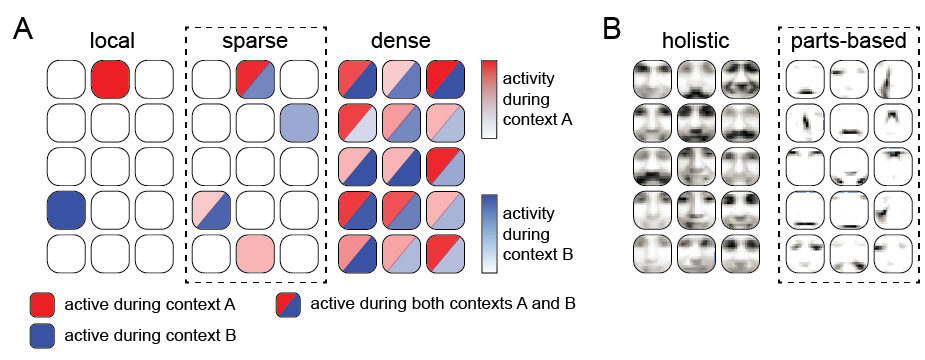
\includegraphics[width=\textwidth]{fig-rev1-sparse}
    \caption{\Acf{NSC} promotes population codes that are both sparse and parts-based.
    \textbf{\emph{A}},
    	   Hypothetical activity in a population of neurons
           during presentation of two different external stimuli (`contexts').
           A sparse code is a trade-off between a local code
           (where a context is represented by the activity of a single neuron,
           and different contexts are represented by different neurons), and a
           dense code (where all neurons are active and their combined activity is
           used to encode each context).
           Dense codes possess great memory capacity, but suffer from cross talk
           among neurons, whereas local codes do not suffer from interference
           but also have no capacity for generalization
           (adapted from \cite{SpanneJorntell2015}).
     \textbf{\emph{B}},
           In a holistic representation of faces, 
           individual neurons in the population
           respond themselves to faces as a whole \cite{TanakaFarah1993},
           whereas in a parts-based representation
           individual neurons explicitly encode individual face components
           \cite{Palmer1977},
           such as the eyes, nose, and mouth
           (adapted from \cite{LeeSeung1999}).}
	\label{fig:sparse-parts}
\end{figure}


Another approach is to reduce the number of
variables required to represent a particular stimulus space;
a process known as
\textbf{dimensionality reduction}.
Dimensionality reduction methods have proved useful in elucidating neural mechanisms
that depend on how the responses of multiple neurons covary,
including odor discrimination in the olfactory system \cite{Broome2006,Koulakov2011},
the selection and integration of sensory inputs 
in the prefrontal cortex \cite{Mante2013},
and the ability of premotor cortex 
to prepare movements without executing them \cite{Kaufman2014}.

In brain areas far removed from sensory input,
neurons typically encode several behaviorally relevant parameters
simultaneously \cite{Rigotti2013,Park2014,PaganRust2014,PougetSejnowski1997},
allowing for multifaceted representations of high-dimensional stimulus spaces.
For example, a population of neurons tasked with encoding human faces
might opt to represent each individual face as a combination of a set of
standard faces (Fig.~\ref{fig:sparse-parts}B, left column).
In such a \textbf{holistic representation} of faces \cite{TanakaFarah1993},
each individual neuron would itself respond to a face as a whole
(i.e., a face `template')
without explicitly representing individual face components,
and an arbitrary face could be represented by 
combining different face templates
(e.g., by adding 10\% of template 1 to 20\% of template 2
and subtracting 30\% of template 3).
On the other hand, faces can also be represented as a combination
of individual face components, such as eyes, noses, and mouth,
in what is known as a \textbf{parts-based representation}
(Fig.~\ref{fig:sparse-parts}B, right column) \cite{Palmer1977}.
Both approaches allow for representing arbitrary faces as a combination of
neural activity, but have drastically different consequences on the
set of stimulus features each neuron responds to.
Although visual information from the eyes, nose, and mouth would of course be
included in a holistic face representation,
that information would not be explicitly represented as structural units
in their own right \cite{TanakaFarah1993}.
Linear combinations of holistic components often involve complex cancellations
between positive and negative contributions,
and thus lack the intuitive meaning of adding parts to form a whole.
In contrast, a parts-based representation allows for only nonsubtractive
combinations of stimulus features \cite{Palmer1977}.
Although the relevant stimulus dimensions are often not known \emph{a priori},
several sophisticated mathematical techniques exist that
allow us to discover these representations directly from experimental data
\cite{Brunton2016,CunninghamYu2014,PillowSimoncelli2006,Sharpee2014,Gao2017}.

In this article, we demonstrate that a variety of neuronal responses
can be understood as an emergent property of efficient population coding
based on dimensionality reduction and sparse coding.
Specifically, we review computational evidence
from data analyses and computer simulations arguing that \ac{NSC}, 
a combination of \textbf{\ac{NMF}}
\cite{PaateroTapper1994,LeeSeung1999} 
and sparse coding,
can generate sparse and parts-based embeddings of
high-dimensional stimulus spaces
that resemble neuronal population responses in a 
wide variety of brain regions.
This introduces the possibility that \ac{NSC} might
be a general principle to which many neuronal computations adhere.
Furthermore, \ac{NSC} might provide a useful theoretical framework under which
to understand the often complex and nonintuitive response properties of neurons
in brain areas far removed from sensory input.

\section*{Nonnegative sparse coding (NSC) as a modern variant of the efficient coding hypothesis}

\subsection*{Efficient coding}

The fundamental principle of \textbf{efficient coding}
is that a sensory system is
adjusted to the specific statistics of the natural environment from which
it encodes and transmits information
\cite{Barlow1961,Attneave1954,Linsker1990,LouieGlimcher2012}.
\revise{Efficiency, in this context, is an information-theoretic term 
that should not be confused with `minimizing energy expenditure'.
Instead, a sensory pathway is treated as a noisy communication channel, where 
the goal is to maximize the rate at which information can be reliably transmitted
by minimizing the redundancy between representational units.}

Early theories of efficient coding
\cite{Barlow1961,Attneave1954}
were developed based on the visual system.
Attneave \cite{Attneave1954} pointed out that there is a significant
degree of redundancy in natural visual images due to correlations in both
the spatial and temporal domains
(for a recent review, see \cite{SimoncelliOlshausen2001}).
For example, the luminance values of a pair of pixels
separated by a fixed distance in a natural image
are likely to be highly correlated
(Fig.~\ref{fig:ech}A).
These statistical regularities constrain the images a visual system
is likely to encounter to a tiny fraction of the set of all
possible images.
It was therefore argued that the visual system should not
waste resources on processing arbitrary images,
but instead use statistical knowledge
about its environment to represent the relevant input space 
as economically as possible.


\begin{figure}[h]
	\centering
% 	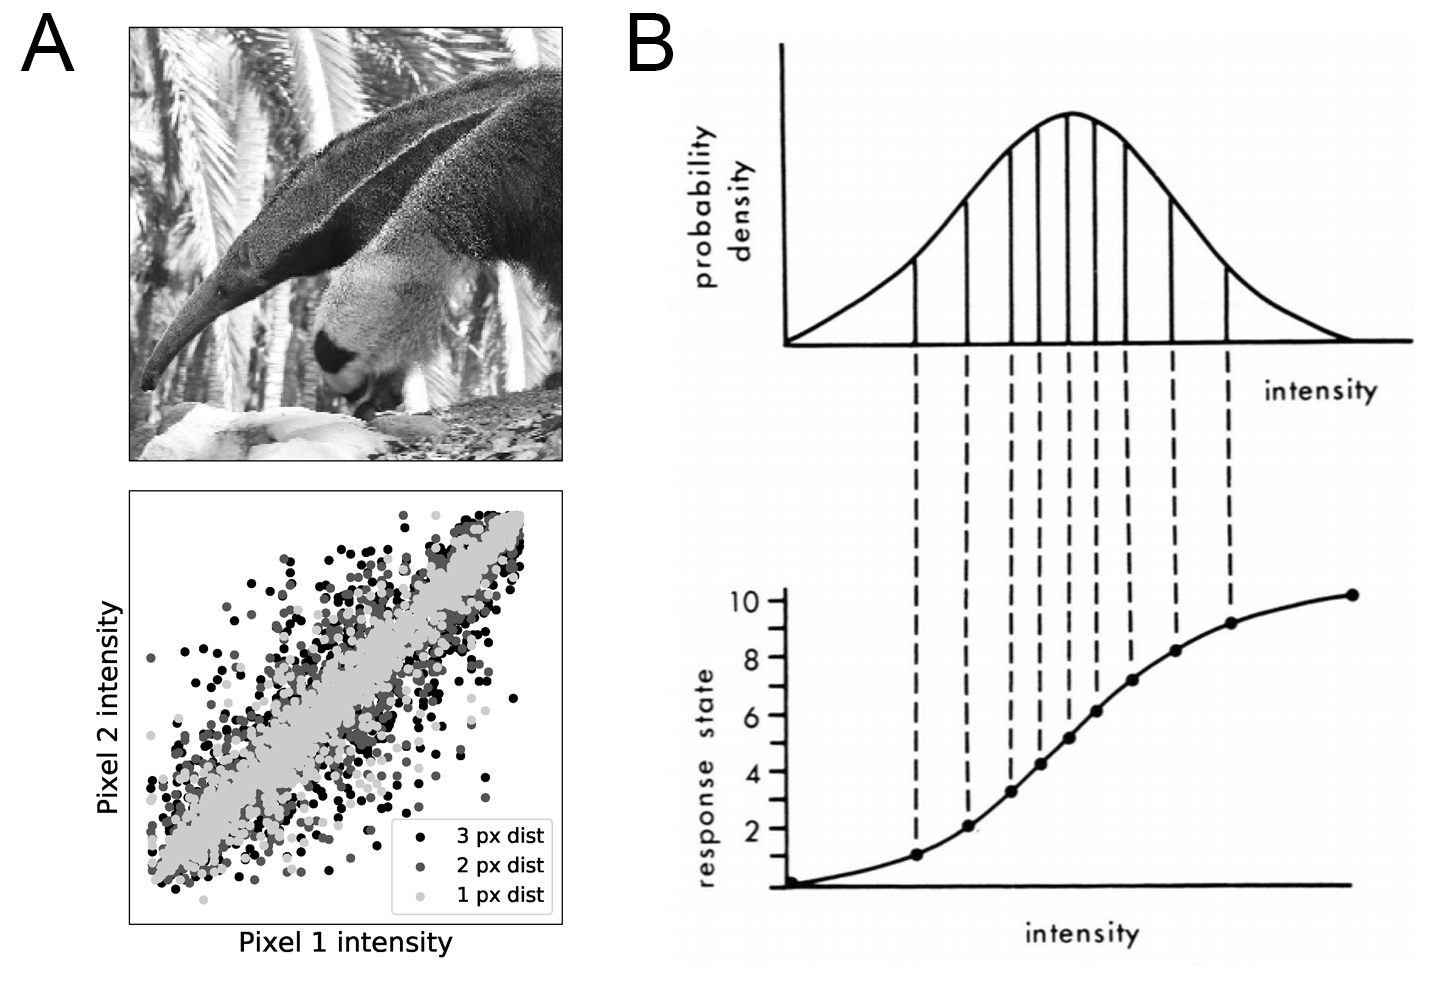
\includegraphics[width=\textwidth]{fig-rev2-ech}
    \caption{Efficient coding hypothesis.
    \textbf{\emph{A}},
         Sensory stimuli in the environment, such as an image of \revise{an anteater},
         display significant statistical structure. For example, the luminance
         value of nearby pixels in the image are significantly correlated,
         an effect that exists even for nonadjacent pixels \revise{(inspired by \cite{LouieGlimcher2012})}.
         Neural systems can improve their coding efficiency by accounting
         for and reducing such information redundancy.
     \textbf{\emph{B}},
         For a given distribution of sensory characteristics in the world \revise{(top)},
         \revise{a neuron's information capacity is maximized 
         when all response levels are used with equal frequency
         (reprinted from \cite{Laughlin1981} under CC-NC-ND 3.0).
         Intervals between each response level encompasses an equal area
         under the intensity distribution, so each state is used with
         equal frequency.}
    }
	\label{fig:ech}
\end{figure}


Extending this idea to the neural level,
Barlow \cite{Barlow1961} proposed that
the goal of early neurons in sensory processing is to remove
the redundancy in the input stimuli.
These ideas were shaped by two
fundamental empirical observations
about early visual cortex:
1) a neuron's \ac{RF} resembled a decomposition of the visual
stimulus into a series of local, largely independent feature components
(e.g., a 2-D Gabor function is basically a local approximation of the
directional spatial derivative of an image),
and 2) any individual neuron responded only sparsely to a small subset of
stimulus features (e.g., orientation or color at a particular spatial location).
Thus a neuron's \ac{RF} could be understood as a
sparse, low-dimensional embedding of high-dimensional input stimuli
\cite{Barbieri2015}.
\revise{However, there is the possibility that sparsity results from a limited stimulus set as we discuss in the ``Model limitations'' section.}

At the level of single neurons, efficient coding requires
that a neuron's input-output function be adjusted so that all
activity levels are used equally in response to a specific
stimulus distribution \cite{Simoncelli2003} (see Fig.~\ref{fig:ech}B).
If the input-output function sensitivity is too low,
high levels of the stimulus feature will be indistinguishable
as the response function saturates; if the sensitivity is set too high,
low levels of the stimulus feature cannot drive responses 
\cite{Laughlin1981}.

At the level of neuronal populations,
neural responses should be both \emph{decorrelated}
(i.e., independent from one another)
and \emph{sparse}
(i.e., involve only a small fraction of neurons in the population)
\cite{LouieGlimcher2012}.


\subsection*{Sparse coding}

Taking these ideas a step further,
Olshausen and Field \cite{OlshausenField1996b} 
noted that natural images contain statistical
dependencies beyond linear pairwise correlations among image pixels,
and argued that these higher-order correlations should be taken into
account when developing an efficient code.
Their goal was thus to find a linear coding strategy
capable of reducing these higher-order forms of redundancy.

\emph{Linear sparse coding} is one such strategy,
where monochromatic images $I(x,y)$
are described in terms of a linear superposition of
a number of \textbf{basis functions},
$w_b(x,y)$:
\begin{equation}
I(x,y) = \sum^B_{b=1} w_b(x,y) h_b,
\label{eqn:sparse-coding}
\end{equation}
where $h_b$ are stochastic coefficients that are different for each image
\cite{OlshausenField1996,Hyvarinen2001}.
Learning a sparse code for images thus involved determining
the values of both $w_b(x,y)$ and $h_b$ for all $b$ and $(x,y)$,
given a sufficient number of observation of images,
under the constraint that $h_b$ be sparse.
In this context, $h_b$ was considered sparse if it took very small
or very large (absolute) values more often than a Gaussian random
variable would \cite{Hyvarinen2001}.
This sparsity constraint allowed for basis functions that were not
needed to describe a given image structure to be weeded out.

\revise{Sparsity, in this context, is an information-theoretic concept
related to how efficiently and completely information is encoded with
the basis functions described above.
Please note that this is different from empirical observations
of brain areas being `sparsely' activated; that is,
sparse population activity does not necessarily imply that a brain area
implements a sparse coding scheme.
This confusion is fueled in part by the wide variety of definitions of sparsity
used in the literature\cite{SpanneJorntell2015,BarthPoulet2012}.}

When Olshausen and Field applied linear sparse coding 
to natural images,
they found that the emerging basis functions 
were qualitatively similar in form
to \acp{RF} of simple cells in \ac{V1} 
\cite{OlshausenField1996,OlshausenField1997},
thus giving empirically observed \acp{RF} 
an information-theoretic explanation.
In this context, $h_b$ in Eq.~\ref{eqn:sparse-coding} above
corresponded to the (signed) activation value of a particular \ac{V1}
neuron, and $w_b(x,y)$ were the connection weights
(or \emph{synaptic weights} in an artificial neural network)
that were closely related to that neuron's \ac{RF}.
Olshausen and Field went on to show that 
the set of basis functions that best described \ac{V1} \acp{RF} 
was greater in number than the effective
dimensionality of the input
(\revise{which they termed} an \emph{overcomplete} basis set) 
\cite{OlshausenField1997}.
\revise{It is worth noting that sparse coding with an overcomplete basis set
is typically associated with an anatomical fan-out motif,
such as expanding 1 million optic nerve fibers 
into more than 100 million \ac{V1} neurons,
or from a small number of mossy fibers to a 100-fold larger number of
granule cells in the cerebellum.}

However, as pointed out by Hoyer \cite{Hoyer2003}, 
linear sparse coding falls short of providing a literal interpretation
for \ac{V1} simple-cell behavior for two reasons:
1) every neuron could be either positively or negatively active, and
2) the input to the neural network was typically double-signed,
whereas \ac{V1} neurons receive visual input from the \ac{LGN} 
in the form of separated, nonnegative ON and OFF channels.

In order to transform Olshausen and Field's sparse coding
from a relatively abstract model of image representation 
into a biologically plausible model of early visual cortex processing,
Hoyer \cite{Hoyer2002,Hoyer2003} thus proposed to enforce
both input signal and neuronal activation to be nonnegative.
This seemingly simple change had remarkable consequences 
on the quality of the sensory representation:
Whereas elementary image features in the standard sparse coding model
could `cancel each other out' through subtractive interactions,
enforcing nonnegativity ensured that features combined additively,
much like the intuitive notion of combining parts to form a whole.
The resulting parts-based representations resembled \acp{RF} in \ac{V1} 
much more closely than other holistic representations.
These considerations led to the formulation of nonnegative sparse coding (\ac{NSC}) in its current form.


\subsection*{Nonnegative sparse coding (NSC)}

As a special case of linear sparse coding,
\ac{NSC} shares the same goal of accurately describing observed data
as a superposition of a set of sparsely activated basis functions.
However, \ac{NSC} additionally requires 
all basis functions and activation values
(i.e., $w_b(x,y)$ and $h_b$ in Eq.~\ref{eqn:sparse-coding})
to be nonnegative.

Consider $S$ observed stimuli or data samples,
each comprised of $F$ observed feature values,
such as a collection of $S$ images $I(x,y)_s$ ($s \in [1, \ldots, S]$)
from the example above,
each consisting of $F$ different grayscale values.
If we arrange the observed feature values of the $s$-th observation into
a vector $\vec{v}_s$ (i.e., by flattening each observed image),
and if we arrange all vectors into the columns 
of a $F \times S$ data matrix \textbf{V},
then linear decompositions describe these data as:
\begin{equation}
\mathbf{V} \approx \mathbf{WH},
\label{eqn:linear-decomposition}
\end{equation}
where \textbf{W} is a $F \times B$ matrix that contains as its columns
the $B$ basis functions of the decomposition
(i.e., the $b$-th column of \textbf{W} corresponding to 
$w_b(x,y)$ $\forall x,y$ in Eq.~\ref{eqn:sparse-coding}),
and \textbf{H} is a $B \times S$ matrix containing
as its columns the activation values 
of each basis function for a particular input stimulus
(i.e., the $b$-th column of \textbf{H} corresponding to 
$h_b$ $\forall b$ in Eq.~\ref{eqn:sparse-coding}).
The difference between \textbf{V} and \textbf{WH} is termed
the \emph{reconstruction error}.

The goal of \ac{NSC} is then to find a linear decomposition of \textbf{V}
that minimizes the reconstruction error,
while guaranteeing that \textbf{H} is sparse.
This can be achieved by minimizing the following cost function
\cite{Hoyer2002}:
\begin{equation}
\min_{\mathbf{W}, \mathbf{H}} \frac{1}{2} ||\mathbf{V} -\mathbf{WH}||^2 + \lambda \sum_{ij} f(\mathbf{H}_{ij}),
\label{eqn:nsc-cost-function}
\end{equation}
subject to the constraints
$\forall ij: \mathbf{W}_{ij} \geq 0$, $\mathbf{H}_{ij} \geq 0$, and
$||\vec{w}_i|| = 1$, where $\vec{w}_i$ denotes the 
$i$-th column of \textbf{W}.
Here, the left-hand term describes the reconstruction error,
whereas the right-hand term describes the sparsity of the decomposition.
The trade-off between accurate reconstruction and sparsity
is controlled by the parameter $\lambda$ ($\lambda \geq 0$), whereas
the form of $f$ defines how sparsity is measured
(a typical choice is the L1 norm on \textbf{H}).
\revise{\Ac{NSC} explicitly discourages statistically inefficient representations,
because strongly accounting for a rare observation 
at the expense of ignoring a more common one stimulus component
would result in an increased reconstruction error.}

In the case of $\lambda = 0$, Eq.~\ref{eqn:nsc-cost-function}
reduces to the squared-error version of \textbf{\ac{NMF}}.
Although \ac{NMF} enforces all elements of \textbf{W} and \textbf{H}
to be nonnegative,
the resulting decomposition might not be sparse,
depending on the number of basis functions $B$.
In order to emphasize decompositions where \textbf{H} is sparse,
Eq.~\ref{eqn:nsc-cost-function} should be minimized 
with $\lambda > 0$ \cite{Hoyer2002}.

Another open parameter is the number of basis functions, $B$, 
which controls the predictive power of the model,
and must be determined empirically.
With a small number of basis functions,
\ac{NSC} is unlikely to achieve a low reconstruction error
be it in familiar contexts (training data) or in novel contexts
(held-out test data).
In this case, the error depends on the systematic bias of the model,
and the model is said to \emph{underfit} the data
(left-hand side of Fig.~\ref{fig:nsc-bias-variance-dilemma}).
With increased model complexity,
the model can learn subtle differences 
between different contexts with high accuracy,
leading to a reduced bias (training) error.
However, with increased complexity, the model is more likely to learn
patterns between training contexts that arise either from underlying noise
or from spurious correlations. As a result,
the model will respond according to
these learned patterns when a novel context is presented
(rather than according to the underlying actual relationships), 
in which case the model is said to \emph{overfit} the data
(right-hand side of Fig.~\ref{fig:nsc-bias-variance-dilemma}).
Hence, the goal of a successful model is to find the ideal compromise
in the bias-variance error trade-off \cite{Beyeler2017}
(labeled `best model' in Fig.~\ref{fig:nsc-bias-variance-dilemma}).

\begin{figure}[h]
	\centering
% 	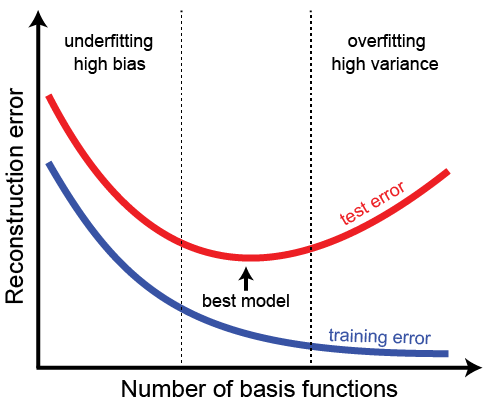
\includegraphics[width=0.6\textwidth]{fig-rev1-bias-variance}
    \caption{The bias-variance dilemma.
    With increased model complexity 
    (i.e., with an increased number of basis functions), 
    the reconstruction error on a set
    of familiar (training) data typically decreases until it reaches zero.
    In contrast, the reconstruction error on a set of unfamiliar, held-out
    (test) data typically goes through a minimum as a function of model complexity.
    A successful model chooses the number of basis functions such that the
    generalization (test) error is minimized (labeled `best model`).}
	\label{fig:nsc-bias-variance-dilemma}
\end{figure}

Analogously to \cite{OlshausenField1996,OlshausenField1997},
the basis functions obtained in \ac{NSC} can be interpreted as
the connection weights of a population of simulated neurons
in an artificial neural network.
In other words, under \ac{NSC} the number of basis functions $B$ 
corresponds to the number of output neurons, and the
response of the $b$-th model output neuron
($b \in [1, ..., B]$)
to a particular input stimulus $s$, termed $r_{bs}$,
can be computed by feeding the dot product of
that neuron's connection weights
(i.e., the $b$-th column in $\mathbf{W}$, $\vec{w}_b$)
and a data vector
(i.e., the $s$-th column in \textbf{V}, $\vec{v}_s$)
to an activation function $\Theta$:
\begin{equation}
r_{bs} = \Theta(\vec{w}_b \cdot \vec{v}_s),
\label{eqn:nsc-model-response}
\end{equation}
where $\cdot$ denotes the dot product.
For example, the linear response of a model neuron
can be calculated by setting $\Theta$ to the identity function $\Theta(x)=x$.
Note that the response of the model neuron to different stimuli 
$s \in [1, \ldots, S]$
involves different columns of \textbf{V},
but always relies on $\vec{w}_b$.

Inhibitory connections can be modeled in the same fashion,
by interpreting inhibitory connection weights
as nonnegative synaptic conductances.
\revise{For example, Hoyer \cite{Hoyer2003} used \ac{NSC} to model \ac{V1} neurons
as receiving input from both excitatory ON and inhibitory OFF cells in the \ac{LGN}.
Using pre-whitened natural images, Hoyer sampled $12 \times 12$ pixel patches from
the images, and then separated positive and negative values into separate channels.
Each image patch was thus represented by a $2 \times 12 \times 12 = 288$ dimensional vector,
each element of which mimicked the activity of an ON or OFF cell
in response to the image patch.
These vectors were then arranged into the columns of \textbf{V}.}
This procedure not only preserved the parts-based quality of the encoding,
but also allowed for more complicated connection types to be modeled.
However, it is interesting to note that a more recent study has argued
that the nonnegativity constraint on the
connection weights might not be necessary 
to preserve the parts-based quality of the encoding (see \cite{Liu2017}).

Thus, we can utilize \textbf{W} 
(which must remain fixed once learned)
and Eq.~\ref{eqn:nsc-model-response}
to simulate a model neuron's response to arbitrary input stimuli
by replacing the column in \textbf{V} with new input.
This allows us to investigate the response properties 
of individual model neurons
much in the same way that experimental neuroscientists 
study biological neurons.
This is important because it means that \ac{NSC} can be used to 
model neural activity in the brain, 
and the resulting activity patterns generated by \ac{NSC}
can be compared to and evaluated against experimental findings. 


\section*{Empirical evidence for nonnegative sparse coding in the brain}

An influential paper by Lee and Seung \cite{LeeSeung1999}
found that applying \ac{NMF} to a database of face images
yielded sparse, localized features that resembled parts of a face
\revise{(Fig.~\ref{fig:NMF|reconstruction}A)}.
In their case, \ac{NMF} acted on a
$F \times S$ data matrix \textbf{V},
whose rows corresponded to distinct features of the input 
(e.g., $F$ different pixels of an image)
and whose columns corresponded to different stimuli or 
observations of those features
(e.g., $S$ different images).
\ac{NMF} was used to decompose the matrix into two reduced-rank matrices
(Fig.~\ref{fig:NMF|reconstruction}, \revise{inset})
whose linear combination could be weighted such that the product of \textbf{W} and \textbf{H} provided an accurate reconstruction of \textbf{V}
\revise{(see Eq.~\ref{eqn:linear-decomposition}).}

A particular image, in this case encoded by $F = 19 \times 19 = 361$ pixels
could be accurately represented by a linear combination of 
a small number ($B = 49$) of encoding variables or `basis images'
(Fig.~\ref{fig:NMF|reconstruction}\revise{A}).
Such a representation is reminiscent to neural processing in \ac{IT},
an area in the ventral visual `what' stream
involved in encoding high-level object identity
\cite{BrincatConnor2004,Majaj2015},
where images of whole faces can be linearly reconstructed
using responses of approximately $200$ neurons
that each respond to a certain set of physical facial features
\cite{ChangTsao2017}.

\begin{figure}[ht]
	\centering
% 	\includegraphics[width=\textwidth]{fig4}
    \caption{\revise{Sparse and parts-based representations recovered by \ac{NMF}
             resemble receptive fields across brain regions.
             \Ac{NMF} (inset) can reconstruct a} data matrix \textbf{V}
             ($F$ features x $S$ stimuli)
             from two reduced-rank matrices \textbf{W}
             (containing $B$ basis functions) and \textbf{H}
             (containing the hidden coefficients of the decomposition).
             Any individual input stimulus (i.e., column in \textbf{V}, \revise{red})
             can be reconstructed from a linear combination
             \revise{(i.e., column in \textbf{H}, blue)}
             of a set of basis functions (i.e., all columns in \textbf{W}, 
             \revise{green}).
         \textbf{\emph{A}},
             A facial image can be reconstructed from a sparse activation
             of simulated \acs{IT} neurons that
             preferentially respond to parts of faces
             (adapted from \cite{LeeSeung1999}).
         \textbf{\emph{B}},
             An optic flow field can be reconstructed from a sparse
             activation of model \acs{MSTd} neurons that prefer various
             directions of 3D self-translation and self-rotation
             (adapted from \cite{Beyeler2016}).
         \textbf{\emph{C}},
             A rat's 2D allocentric position and route-based direction of
             motion can be reconstructed from a sparse activation of
             model \acs{RSC} neurons that prefer an intricate combination of
             linear velocity (LV), angular velocity (AV), head direction (HD)
             and 2D position (P).
             For the sake of clarity, only the 4 most contributing hidden
             coefficients (out of 30) are shown.}
	\label{fig:NMF|reconstruction}
\end{figure}


\revise{Interestingly}, such a parts-based representation is not specific to
information processing in \ac{IT};
the same principle can be extended to other areas of the visual system,
such as the \ac{MSTd},
which is part of the visual motion pathway \cite{Beyeler2016}.
Neurons in \ac{MSTd} respond to relatively large and complex patterns
of retinal motion (`optic flow'),
owing to input from direction and speed selective neurons in the \ac{MT}
(for a recent review, see \cite{Orban2007}).
Although \ac{MSTd} had long been suspected to be involved in the
analysis of self-motion,
the complexity of neuronal response properties has made it difficult
to experimentally investigate how neurons in \ac{MSTd}
might perform this function.
However, when \revise{our group} 
applied \ac{NMF} to 
\revise{simulated neural activity patterns whose statistical properties
resembled that of experimentally recorded \ac{MT} neurons} 
\cite{Beyeler2016},
\revise{we} found a sparse, parts-based representation of retinal flow
(Fig.~\ref{fig:NMF|reconstruction}\revise{B})
similar to the parts-based representation of faces
encountered by Lee and Seung \cite{LeeSeung1999}.
The resulting `basis flow fields' showed a remarkable resemblance to receptive fields
of \ac{MSTd} neurons, as they \revise{responded to}
an intricate mixture of
3D translational and rotational flow components
in a subset of the visual field.
As a result, any flow field possibly to be encountered 
during self-movement through a 3D environment
could be represented by only $B = 64$ simulated \ac{MSTd} neurons,
as compared to $F = 9,000$ simulated \ac{MT} input neurons.
This led to an sparse \revise{and parts-based} population code,
where any given stimulus could be represented
by only a small number of simulated \ac{MSTd} neurons
\cite{Beyeler2016}.

Analogously, \ac{NSC} can explain response properties
of neurons outside the visual system, 
such as in the \ac{RSC}, an area in the posterior cingulate region
important for navigation and spatial memory \cite{Miller2014,Nelson2015,VannAggleton2009}.
Neurons in the \ac{RSC} conjunctively encode multiple variables related to the environment and one's position and movement within it
\revise{(e.g., position, head direction, linear velocity, and angular velocity)},
allowing the representation of spatial features of the environment 
with respect to multiple reference frames \cite{AlexanderNitz2015}.
\revise{When our group applied \ac{NMF} to neurophysiological data from
\ac{RSC} neurons while rats ran back and forth on a W-shaped track
(for experimental details, see Supplementary Materials),
we again found a sparse and parts-based representation for behaviorally
relevant variables such as the animal's position, head direction, 
and movement direction (Fig.~\ref{fig:NMF|reconstruction}C).
Interestingly, model \ac{RSC} neurons encoded these variables with respect
to multiple frames of reference
(e.g., head direction: \textbf{allocentric reference frame},
linear velocity: \textbf{route-based reference frame}).
Once again, the dimensionality of the stimulus space was drastically reduced
from $F = 417$ input neurons to a set of $B = 30$ model \ac{RSC} neurons.}

\revise{Due to its roots in efficient-coding theories of natural image processing,
there is a large body of research highlighting the role of \ac{NSC} in
visual cortex function
(e.g., \cite{Barlow1961,OlshausenField1996,Hoyer2003,BenHamed2003}).}
Although there seems to be a consensus that 
information-theoretic explanations are relevant 
when investigating the early visual system,
higher-order brain areas are often considered to be specialized for
performing tasks
(e.g., recognizing objects, making decisions, navigating an environment),
rather than the efficient encoding of information.

\revise{However, more recently, 
\ac{NSC}-like computational models have found application outside visual cortex,
where they have started to provide compelling evidence that a wide variety of
neuronal response properties can be understood as an epiphenomenon
of efficient population coding based on dimensionality reduction.
Examples include elucidating the dimensions along which perceptual space
is organized in the olfactory system
\cite{MorenoBoteDrugowitsch2015,Castro2013},
the coordination of movement in the cortico-basal ganglia-thalamo-cortical loop
\cite{BarGad2000,BarGad2003_Review},
and the combined representation of allocentric and route-based 
spatial navigation cues
in retrosplenial cortex \cite{Rounds2018}.}
\revise{The success of these models suggests that \ac{NSC}}
might apply elsewhere in the brain, 
\revise{thus warranting further investigation.}
In fact, sparse (and potentially parts-based) representations have been observed
in \revise{a wide variety of brain areas}
(see Table~\ref{table:listEvidence}).
This introduces the \revise{intriguing} possibility that \ac{NSC} might
be a general principle to which \revise{many} neuronal computations adhere.
\revise{In the future, \ac{NSC} might provide a useful theoretical framework
under which to understand the often complex and nonintuitive response properties
of neurons in brain areas far removed from sensory inputs,
including the selection and integration of various task-related variables
in prefrontal cortex
\cite{Mante2013}
and the ability of premotor cortex to prepare movements without executing them
\cite{Kaufman2014}.}



\begin{table}[ht]
\begin{adjustwidth}{-2.25in}{0in}
	\centering
	\caption{Nonnegative sparse coding in the brain.
    We list a group of brain regions for which there is experimental evidence of certain features associated with NSC (`X': evidence exists, `?': has yet to be investigated).
   For each brain region, the left-hand side of the table lists experimental evidence for sparse \revise{population codes} and/or parts-based representations, whereas the right-hand side lists computational support that \revise{\ac{NSC}-like models} can describe receptive fields or response properties within that region.}
    \def\arraystretch{1.1}
    {\setlength{\tabcolsep}{1em}
    \begin{tabular}{r|rrr|rr}
	\revise{\textbf{Brain}} & \textbf{Sparse} &  \textbf{Parts-} & \textbf{Experimental} & \textbf{Modeled} & \textbf{Computational} \\
	\textbf{Area} & \revise{\textbf{code}} & \textbf{based} & \textbf{evidence} & \textbf{by NSC} & \textbf{ support} \\ \hline
    Retina & X & X & \cite{Onken2016,Liu2017} & X & \cite{Onken2016,Liu2017} \\
    \revise{Visual cortex} & X & X & \pbox{5cm}{\cite{OlshausenField1996,HoyerHyvarinen2002,vanHateren1998,Wachsmuth1994,FreiwaldTsao2010,ChangTsao2017,BenHamed2003}} & X & \pbox{5cm}{\cite{OlshausenField1996,Hoyer2003,Carlson2013,Hyvarinen2001,LeeSeung1999,Hosoda2009,Beyeler2016}} \\
    Auditory cortex & X & \revise{X} & \revise{\cite{Hromadka2008,rokem2006,bendor2008,Leaver2010,Terashima2013,SmithLewicki2006}} & \revise{X} & \revise{\cite{Martinez2015,David2007}} \\
 	Olfactory cortex & X & \revise{X} & \cite{Koulakov2011,poo2009,rinberg2006,Broome2006,Castro2013} & \revise{X} & \revise{\cite{MorenoBoteDrugowitsch2015,Castro2013}}  \\
 	\revise{Somatosensory} cortex & X  & \revise{X} & 			   \revise{\cite{Jadhav2009,oconnor2010,Crochet2011,Ramirez2014,penfield1937,hari1993,petersen2007}} & \revise{X} & \revise{\cite{WhitewayButts2017,Hafner2004}}  \\
    \revise{Parietal cortex} & \revise{?} & \revise{X} & \revise{\cite{Poggio1990,PougetSejnowski1997,andersen1997multimodal,PougetSnyder2000,louie2015adaptive}} & \revise{?} & \revise{?}  \\
    Retrosplenial cortex & \revise{?} & X & \revise{\cite{AlexanderNitz2015,vedder2016,mao2017}} & X & \cite{Rounds2018} \\
    \revise{Prefrontal cortex} & \revise{?} & \revise{?} & \revise{\cite{Mante2013,Rigotti2013,Fujisawa2008,Wei2015}} & \revise{?} & \revise{?}  \\    
    Motor cortex & \revise{?} & \revise{?} & \revise{\cite{Beloozerova2003,penfield1937,GrazianoAflalo2007,Brecht2004}}
    & ? & \revise{?} \\
    Hippocampus & \revise{X} & \revise{?} & \revise{\cite{ThompsonBest1989,Bakker2008,myers2011pattern,rolls2013,Wixted2014,Poli2017}} & \revise{?} & \revise{?} \\        
    Basal ganglia & X & ? & \cite{BarGad2003_Review,Turner2000,schwab2015} & X & \pbox{5cm}{\cite{BarGad2000,BarGad2003_Review}} \\  
	\end{tabular}}
    \label{table:listEvidence}
\end{adjustwidth}
\end{table}

\revise{In the following subsections,
we review existing experimental evidence
for sparse and parts-based representations 
in various brain areas highlighted in Table~\ref{table:listEvidence}.
Where available, we highlight \ac{NSC}-like computational models
that  successfully explain response properties of individual neurons
or have been instrumental in elucidating the dynamics at the population level.}


\subsection*{Understanding neuronal response properties within the framework of NSC}

\mikeNote{This first subsection is so basic and integral to understanding how NMF maps to neurons that it would almost make sense to move it to subsection ``Nonnegative sparse coding'' in the background section. We would probably add a figure there that shows the NMF schematic V=WH and Fig.4 panel A, so that the reader immediately understands the processing pipeline of how to go from W in NMF to $r_bs$.}

By interpreting the elements of \ac{NMF}'s
matrix \textbf{W} as the synaptic weights of model output neurons,
\ac{NSC} allows for the computation of neuronal response properties
with
methods similar to the ones employed by experimental researchers to understand biological neurons,
and by theoretical neuroscientists to understand computational models. This is important because it means that NSC can be used to model neural activity in the brain, and the resulting activity patterns generated by NSC can be compared to and evaluated against experimental findings. 

In \ac{NSC}, the number of basis functions $B$ corresponds to the number of output neurons. The response of the $b$-th model output neuron
($b \in [1, ..., B]$)
to a particular input stimulus $s$, $r_{bs}$,
can be computed by feeding the dot product of the neuron's presynaptic connections
(i.e., the $s$-th column in \textbf{V})
and the corresponding synaptic weights
(i.e., the $b$-th column in $\mathbf{W}$)
to an activation function $\Theta$
(Fig.~\ref{fig:NMF|neuronalresponse}A).
For example, the linear response of a model neuron
can be calculated by setting $\Theta$ to the identity function $\Theta(x)=x$.
Note that the response of the model neuron to different stimuli 
$s \in 1, \ldots, S$
involves different columns of \textbf{V},
but always relies on the same weight matrix \textbf{W}.
Thus, we can utilize \textbf{W}
(which must remain fixed once learned with \ac{NMF})
to simulate a model neuron's response to arbitrary input stimuli
by replacing the column in \textbf{V} with new input.
This allows us to investigate the response properties of individual model neurons
much in the same way that experimental neuroscientists study biological neurons.

\begin{figure}[h]
	\centering
	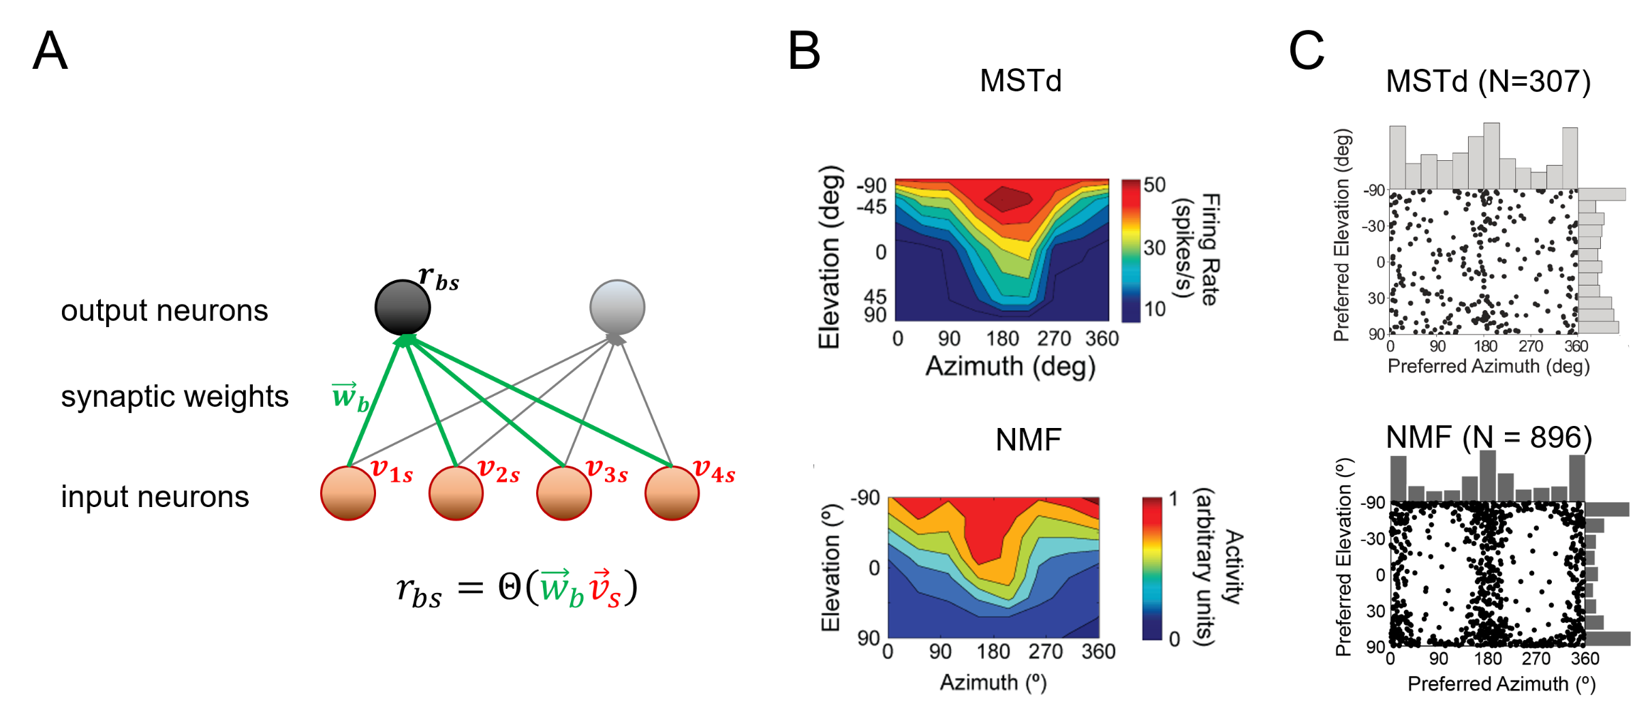
\includegraphics[width=\textwidth]{fig-rev1-responses}
    \caption{\ac{NSC} can predict response properties of biological neurons.
    A) $r_{bs}$ is the response of the $b$-th model output neuron
       to the $s$-th stimulus. $r_{bs}$
       can be calculated from the activity of all
       input neurons (i.e., column $s$ in \textbf{V}), the
       corresponding synaptic weights (i.e., column $b$ in
       $\mathbf{W}$), and a neuronal activation function $\Theta$.
    B) Example of 3D heading tuning for a neuron in macaque
       \ac{MSTd} (top, reprinted from \cite{Takahashi2007}) and a
       simulated neuron (bottom,
       based on the linear response using $\Theta(x)=x$,
       reprinted from \cite{Beyeler2016}).
       Color contour maps show the mean firing rate or model
       activation as a function of azimuth and elevation angles
       of the self-movement direction in 3D.
    C) Classifying simulated akin to biological neuronal responses
       yields distributions of 3D heading preferences akin to 
       macaque \ac{MSTd} (top, reprinted from \cite{Beyeler2016}).
       Each neuron also responded to a preferred direction of 3D
       self-rotation (not shown).}
	\label{fig:NMF|neuronalresponse}
\end{figure}




\subsubsection*{\revise{Visual system}}

\revise{Due to the long history of sparse and efficient coding in vision neuroscience,
the literature is ripe with examples of sparse and parts-based representations
that are in agreement with \ac{NSC}.}

\revise{For example, an \ac{NMF} based model was able to reconstruct
neuronal spike trains in the salamander retina \cite{Onken2016}.}
Following testing on ground truth data, the researchers recorded spikes from in vitro retinal ganglion cells  while the cells were exposed to natural scenes (either still photographs or videos).
They then applied several factorization methods to the data. 
Space-by-time NMF could decompose the data into separate spatial and temporal modules that yielded sparser and more compact representations compared to other techniques, including orthogonal Tucker-2 and basic \ac{NMF}.
\mikeNote{But what does that all mean? Space-by-time NMF? Tucker-2?}
% NMF can also describe patterns of activation observed in retinal ganglion cells (RGCs), which exhibit specific response times and latencies in response to natural images that allow the retina to encode spatial and temporal information embedded in the stimuli. A specific form of NMF, called Tucker-2 or space-by-time NMF, produces separate spatial and temporal basis vectors that most accurately and sparsely describe the spike trains produced by RGCs in the salamander retina \citep{Onken2016}. Nonnegativity constraints, possibly in conjunction with other statistical constraints dependent on the brain region the neurons operate in, may describe the response patterns of neurons in other brain regions that have yet to be tested.


\revise{As discussed above, \ac{NSC} was first demonstrated on simple and
complex cells in \ac{V1} \cite{HoyerHyvarinen2002,Hoyer2003}.
Later, they also modeled V2 hypercomplex cells \cite{Hyvarinen2005}.}
\mikeNote{Expand}

\revise{In our own work \cite{Beyeler2016}, 
we found that simulated neurons in an \ac{NMF} based model 
of \ac{MSTd} responded to simulated optic flow fields
that mimic natural viewing conditions
in much the same way as real neurons in macaque \ac{MSTd}
(Fig.~\ref{fig:NMF|neuronalresponse}B).}
Not only did individual units match response properties of individual neurons
in macaque \ac{MSTd},
but the model was able to recover statistical properties of the \ac{MSTd}
population as a whole, such as a relative overrepresentation of lateral
headings (Fig.~\ref{fig:NMF|neuronalresponse}C).


\subsubsection*{\revise{Auditory cortex}}

\revise{Outside the visual stream, there's lots more stuff.}

http://www.physiology.org/doi/abs/10.1152/jn.00891.2005
\mikeNote{Expand}



\revise{\subsubsection*{Sensory cortex}}
* Evidence from barrel cortex in rats (Spatial organization of neuronal population responses in layer 2/3 of rat barrel cortex)
\mikeNote{If you come across a good figure for any of these areas, I think it would really help us appear more balanced (i.e. less focused on our own work).}

* Auditory cortex (Sparse representation of sounds in the unanesthetized auditory cortex)

* Olfactory cortex (Sparse Incomplete Representations: A Potential Role of Olfactory Granule Cells) and (Causal inference and explaining away in a spiking network)
* Somatosensation?


\revise{\subsubsection*{Motor system}}
* Would it be appropriate to put basal ganglia here? (Information processing, dimensionality reduction and reinforcement learning in the basal ganglia) and (Reinforcement-driven dimensionality reduction–a model for information processing in the basal ganglia)
\mikeNote{Sure, if it flows nicely. Otherwise just make two subsections `basal ganglia' and `motor cortex'.}

* Motor cortex (Rethinking Cortical Organization),(Corticostriatal activity in primary motor cortex of the macaque),(Decoding complete reach and grasp actions from local primary motor cortex populations)


a model known as Reinforcement-Driven Dimensionality Reduction (RDDR)
\mikeNote{revise}
successfully used Hebbian learning to reproduce basal ganglia response patterns associated with reward \cite{BarGad2000}, a function associated with cortico-striato-pallidal circuitry. The authors later applied nonnegativity constraints to the Hebbian learning in the model so that it effectively performed \ac{NMF} on its inputs. The model advanced understanding of the cortico-striato-pallidal loop by capturing behavior of the circuit while explaining the existence of convergent and lateral connections in the region that other models have historically ignored \cite{BarGad2003_Review}. The authors suggest that the basal ganglia uses unsupervised, reward-driven learning to perform dimensionality reduction on cortical inputs for the efficient compression of information in order to plan upcoming actions in the frontal cortex.


\subsubsection*{\revise{Retrosplenial cortex - maybe Archicortex instead?}}
* Hippocampus and Dentate Gyrus (Sparse and specific coding during information transmission between co-cultured dentate gyrus and CA3 hippocampal networks)

* RSC


Analogously, \ac{NSC} can explain response properties
of neurons outside the visual system, 
such as in the \acf{RSC}, an area important for navigation and spatial memory \cite{Miller2014,Nelson2015,VannAggleton2009}.
Neurons in the \ac{RSC} conjunctively encode multiple variables related to the environment and one's position and movement within it, allowing the representation of spatial features of the environment with respect to multiple reference frames \cite{AlexanderNitz2015} (for experimental details, see Supplementary Materials). 

%as determined by an experiment in which rats ran back and forth on a W-shaped track that occupied two different spatial locations within the room in each recording session to test sensitivity to the allocentric reference frame (i.e., track positions $\alpha$ and $\beta$). Outbound and inbound runs were made up of opposite turn sequences (left-right-left (LRL) and right-left-right (RLR), respectively) that corresponded to different sets of trials, which allowed assessment of sensitivity to the egocentric and route-based reference frames. 

However, establishing a mechanistic link between physiological response properties of \ac{RSC} neurons and their underlying representations of space has proved difficult, due to the complexity of their response properties and because inputs to the region are not easily isolated.


We applied NMF to recorded data from the original \ac{RSC} experiment conducted by
Alexander and Nitz \cite{AlexanderNitz2015}. 

%During the experiment, activity from 228 \ac{RSC} neurons was recorded along with four behavioral metrics: linear velocity, angular velocity, head direction, and allocentric position. Using Gaussian and cosine tuning curves, we created idealized input neurons that encoded these four variables. 

By applying \ac{NMF} to the \revise{idealized neural activity}, we were able to replicate
functionality observed in the biological \ac{RSC} (Fig.~\ref{fig:NMF|reconstruction}\revise{C}).
Once again, the dimensionality was reduced from a set of $F = 417$ input neurons to a set of $B = 30$ basis functions.
% \mikeNote{Too soon?}
% The same results were obtained when evolutionary algorithms 
% were used to optimize the metaparameters associated with \ac{STDPH}
% on a population of \acp{SNN} that replicated 
% the same dataset \citep{Rounds2016}.


%    In the case of the \ac{RSC}, the basis vectors that resulted from the NMF model produced activation patterns that could be used to infer behavior, suggesting that the model functions in a manner similar to the biological RSC. Because this region responds to multiple spatial frames of reference (egocentric, route-centric, and allocentric) simultaneously, it is possible to accurately reconstruct the position of an animal within a route situated in a specific part of the environment if neural activity for that route is compared with itself. In contrast, if neural activity associated with the same route but situated in different parts of the room are compared, then the reconstruction of position should be poor (for more details, see \citep{AlexanderNitz2015}), showing that the \ac{RSC} distinguishes routes that have different allocentric positions in space. We found that the activity patterns computed using the NMF basis vectors yielded qualitatively similar results when subjected to the same analysis.

% The results were also consistent for the \ac{RSC}. In the neurophysiological dataset, experimentally observed neurons were classified into three broad categories: 
% % these 3 are so incredibly, excruciatingly wordy 
% 1) those that were insensitive to turn-based actions performed by the rats running along the track but nonetheless exhibited complex and robust firing patterns, 2) those that were sensitive purely to turning behaviors performed by the rats such that they responded exclusively to left or right turns, and 3) neurons that demonstrated turn type selectivity, but with increased firing associated with specific instances of the preferred turn type based on their position in the turn sequence associated with the route regardless of the route's location in allocentric space. When \ac{NMF} was applied to the behavioral variables encoded by idealized input neurons, the resulting basis vectors could be categorized into the same functional categories and followed the same approximate distributions as in the experimental dataset (Fig.  \ref{fig:NMF|neuronalresponse}B).


% In the case of the \ac{RSC}, the basis vectors that resulted from the NMF model produced activation patterns that could be used to infer behavior, suggesting that the model functions in a manner similar to the biological RSC. Because this region responds to multiple spatial frames of reference (egocentric, route-centric, and allocentric) simultaneously, it is possible to accurately reconstruct the position of an animal within a route situated in a specific part of the environment if neural activity for that route is compared with itself. In contrast, if neural activity associated with the same route but situated in different parts of the room are compared, then the reconstruction of position should be poor (for more details, see \citep{AlexanderNitz2015}), showing that the \ac{RSC} distinguishes routes that have different allocentric positions in space. We found that the activity patterns computed using the NMF basis vectors yielded qualitatively similar results when subjected to the same analysis.






% The sparsity and nonnegativity constraints of the \ac{NSC} seem to extract similarities between neuronal firing patterns that result in
% consistent and stable representations, 
% while other statistical methods of dimensionality reduction 
% instead extract differences in firing patterns, thus capturing underlying representations of the data that are less stable and consistent, and are often less sparse. However, the exact implementation of dimensionality reduction in any given part of the brain might vary with the structure, and connectivity of the region.









These remarkable findings where \ac{NSC} can account for neuronal response properties across a wide range of
brain areas and modalities strongly suggests that these 
 representations emerge due to the pressure to find efficient, perceptually and behaviorally relevant stimulus features.
At the population level, \ac{NSC} promotes representations in which
neurons act as generalists rather than specialists,
allowing for the simultaneous encoding of multiple variables of interest
(e.g., heading, eye rotation velocity in \ac{MSTd} \cite{Beyeler2016})
with respect to multiple frames of reference
(e.g., egocentric, route-based in \ac{RSC} \cite{Rounds2016}).
Among the advantages of such basis function representations
\cite{Poggio1990,PougetSejnowski1997,PougetSnyder2000}
(also called mixed-selectivity representations
\cite{Eichenbaum2017,Fusi2016,Barak2013})
are robustness to noise as well as the ability to decode various variables of interest
through a linear combination of neuronal responses.

% The fact that  \ac{NSC} can account for the response properties of neurons in a diverse set of brain regions that play fundamentally different roles in behavior and cognition is somewhat astounding since individual brain regions are often assumed to have their own unique methods of handling their unique inputs. Evidence for the prevalence of such a computation raises some fundamental questions about how neurons have evolved to help us survive. In particular, these findings suggest that neurons are not, in fact, specialized for particular kinds of computations or functionality, and that it is more advantageous for neurons to be capable of handling all information flexibly. Several researchers have argued that 'mixed selectivity' is a fundamental feature of neurons in higher cortical regions \citep{Eichenbaum2017,Fusi2016,Barak2013}, because higher cognition requires that neurons encode multiple task-relevant variables. Such generalizability is an expected property of neurons under the NSC framework, since the algorithm aims to encode as much information about the stimulus as possible while using the fewest number of neurons to do it. If optimizing these metrics, it is expected that neurons would not be specialized for certain behaviors or inputs, and would instead be equally likely to respond to all types of inputs. This is further supported by evidence showing that sparsity levels amidst populations of neurons demonstrating mixed selectivity helps to control the tradeoff between generalization and discrimination \citep{Barak2013}.


\subsection*{Potential neural mechanisms of NSC}

That \ac{NSC} can explain and reproduce response properties observed in biological neurons may be an important clue as to how brains have evolved to parse and store information
\revise{in order to perceive and interact with the world}.

\revise{Although it is completely possible that neural circuits become connected in some way that NMF or other types of dimensionality reduction just emerges, there are a number of potential neural mechanisms that might implement \ac{NSC}. Here we discuss a few.}
\mikeNote{Words}


\subsubsection*{\revise{Ecology of wiring and stuff}}

\revise{Jeff wanted us to talk about pruning and maybe even the Laughlin work talking about minimizing of wiring. He was on the fence whether we should talk about neural Darwinism.}
\mikeNote{Words}

\revise{Laughlin and Sejnowksi (2003) is a good starting point: They talk about the ecology of wiring, how long-range connections are reconfigured to maximize volume while minimizing area, how to cut down on traffic, etc. These evolutionary pressures might favor NSC-like representations. }


\subsubsection*{\revise{Synaptic plasticity}}

\revise{Then there is the possibility that neurobiological mechanisms might implement a biological equivalent of dimensionality reduction.}
\mikeNote{Words}

One candidate \ac{NSC} process in the brain is synaptic plasticity
which, similar to \ac{NSC},
may act on synapses for the purpose of reducing dimensionality on an input space in order to represent it efficiently and sparsely.
Specifically, we propose that \ac{NSC} might be functionally equivalent to \ac{STDPH}.

\Ac{STDP} is a form of Hebbian learning in which synaptic weight changes depend on the relative timing between pre- and post-synaptic spikes
\cite{BiPoo1998,SongAbbott2000}.
If pre-synaptic spike counts integrated over a critical window precede those of the post-synaptic neuron, then long-term potentiation is induced, strengthening the weight over a time course of milliseconds to seconds. Otherwise, long-term depression is induced, suppressing the weight. \Ac{STDP} is ubiquitous throughout the brain across the lifespan and can take on different forms \cite{Caporale2008STDP,Holtmaat2009STDP}.
%
Homeostasis acts to keep neuronal activity in a good working range \cite{Watt2010}
and to facilitate synaptic competition by normalizing the inputs to a neuron \cite{chistiakova2015},
acting across synapses of a single neuron and across multiple neurons
over a time course of minutes to days
\cite{turrigiano1998}.
One particular form of homeostasis, synaptic scaling, multiplicatively scales weights up or down
depending on the average firing rate of the postsynaptic neuron, which has
been demonstrated to stabilize \ac{STDP} \cite{Carlson2013,Buonomano2005,VanRossum2000}.

Experimental and theoretical evidence suggest that biological processes, such as synaptic plasticity and homeostatic mechanisms, may be reducing the dimensionality of inputs in a similar way to \ac{NMF}
\cite{Perrinet2010,Clopath2010,IzhikevichDesai2003}.
For example, Carlson and colleagues \cite{Carlson2013} provided a mathematical proof that
\ac{STDP} in combination with homeostatic synaptic scaling (i.e., \ac{STDPH})
can approximate the \ac{NMF} algorithm:
Given an input layer of neurons (represented by matrix \textbf{V}) connected to a single output layer neuron (represented by row vector $\vec{h}^T$), \ac{STDPH} iteratively updates the synaptic weights in $\vec{w}$ in such a way as to minimize the reconstruction error of $|\mathbf{V} - \vec{w} \vec{h}^T|$.
Similar to Oja's rule \cite{Oja1982}, which was developed to stabilize 
rate-based Hebbian learning
(effectively resulting in principal component analysis),
synaptic scaling acts as a homeostatic mechanism to stabilize \ac{STDP}
(effectively resulting in \ac{NMF}).
In addition, sparsity of the encoding might be enforced by spike thresholding \cite{Rozell2008} and lateral inhibitory connections \cite{Coultrip1992}.
% Interestingly, popular implementations of \ac{NMF} (e.g., MATLAB, scikit-learn) include a constraint on the L1 norm of \textbf{H} that automatically lead to sparsity. Alternatively, an explicit sparsity level can be incorporated into models of \ac{NMF}, such as in Hoyer's model \cite{Hoyer2004}.

This finding suggests that neurons are able to find accurate factorial
representations of their input stimulus spaces through means of Hebbian-like
synaptic learning. 
\mikeNote{TODO: clarify}
% \emilyNote{moved details to place where experiment is first described, but provide brief overview of STDPH and NMF experiment setups}
To investigate this equivalence
in a more realistic setting,
we conducted simulations in which a model constructed using \ac{STDPH}
and a model constructed using \ac{NSC}
were applied to a dataset of recorded neuronal activity 
observed in the \ac{RSC} of rats in a  spatial navigation task 
(as shown for \ac{NSC} in Figure 1B3). 
In the \ac{STDPH} experiment, the idealized input neurons generated spike trains as input to a population of \acp{SNN} that were trained using an evolutionary algorithm
to match the recorded electrophysiological data \cite{Rounds2016}.
Simulations were performed using CARLsim \cite{BeyelerCarlsonChou2015}, a \ac{SNN} simulator that incorporates a plugin \cite{Carlson2014} to the Evolutionary Computation in Java (ECJ) library \cite{white2012}.

% \jeffNote{I think you can delete the next paragraph. Understanding how EAs work is beside the point. Also, why do you say there is a 3 figure limit?}
% \textcolor{blue}{Evolutionary algorithms are a class of optimization algorithms loosely based on concepts from evolution. A set of individuals (in this case, \acp{SNN}) have a set of parameters, which are to be evolved by repeatedly undergoing a training and a testing phase followed by evaluation that measures how well individuals in the population meet the desired criteria (i.e., their \emph{fitness}; usually determined through a user-defined function).
% A number of individuals are then chosen as parents for the next generation, which can undergo \emph{crossover} (i.e., where a child inherits parameters from its parents whose values have been swapped at random) and/or \emph{mutation} (i.e., where a child inherits parameters from its parents with values randomly chosen from a distribution of values) to produce a new generation of individuals. This process continues until the fitness of the population no longer improves.}

In the experiments in which \acp{SNN} were tuned to replicate \ac{RSC} neurophysiological data, \ac{STDPH} parameters in the model were evolved in an indirect encoding paradigm \cite{Rounds2016}. During each generation of the evolutionary run, \acp{SNN} were subject to \ac{STDPH} learning on trials selected from the available dataset, then \acp{SNN} were tested with \ac{STDPH} turned off on trials selected from trials reserved for testing. At the end of each generation, \ac{SNN} activity 
\mikeNote{TODO Rev1: were the correlations high?}
was correlated with electrophysiologically recorded neural activity, which served as the fitness metric for the algorithm. The \ac{STDPH} parameters were mutated according to an evolutionary strategy and a new population of \acp{SNN} was trained and tested in the following generation.

\mikeNote{TODO Rev1: Add a schematic of the network architecture? It might make more sense to put this in the Supplements}
In the \ac{NSC} experiment, the idealized \revise{neural activity}
was used to construct a matrix of training data associated with each of the four recorded `features' (i.e., linear velocity, angular velocity, head direction, and position), to which \ac{NMF} was applied.



% Half of the trials from each recording session in the dataset were used for training, while the latter half were reserved for testing. \emilyNote{said this in Box 3}
% \mikeNote{IMO these following paras are much too detailed. I think the EA details distract from the main argument, and don't add much value for the general understanding. The reader doesn't need to understand binary tournament selection, crossover, and mutation to appreciate the fact that you were able to fit SNN activity to neurophysiological recordings. Also now the glossary is 44\% EAs.}
% In these experiments, the
% \mikeNote{What population?}
% population size was $N = 15$. We randomly selected trials from a pool containing half the trials in the dataset for training (the other half were reserved for the testing phase). The testing phase was the same as the training phase except STDPH was disabled. Following testing, we measured correlations between synthetic and electrophysiological activity patterns and chose synthetic neuronal matches for each experimentally observed firing pattern based on the best correlations between them. Following fitness evaluation, we used
% \mikeNote{IMO could be shortened. ``We used an evolutionary strategy (binary tournament selection, mutation without crossover) implemented in CARLsim [REF] and ECJ [REF] to match this to that.'' or similar. }
% \textbf{binary tournament selection} to choose three new parents (each parent produced five children) for the next generation of individuals. Each new parent underwent mutation without crossover to produce a new child.
% To compare experimental neuronal responses with synthetic ones, we analyzed functional neuron types using methods described in Alexander and Nitz \citep{AlexanderNitz2015}. Activations averaged over trials for every neuron in the population were cross-correlated to reconstruct agent’s position within a route. To reconstruct position with respect to one route (such as in 
% \mikeNote{Please first explain what $\alpha$ and $\beta$ are. L and R are a bit easier to guess}
% $\alpha$LRL), trials were divided into two sets, even and odd, to measure consistency of response. To reconstruct position between track positions (such as in $\alpha$$\beta$LRL), activations over trials associated with the $\alpha$ track position were averaged and cross-correlated with averaged activations over trials associated with $\beta$. High correlations between same positions (e.g., bin 1 (row) and bin 1 (column)) indicate a good reconstruction of position from ensemble activity
% \mikeNote{add ``see Fig. X, Y'' etc.?}
% patterns. Within-position reconstructions (even vs. odd trials) yielded accurate positional reconstructions (low error), but between-position (i.e., $\alpha$ vs. $\beta$ trials) were associated with high error and did not yield accurate reconstructions of position, which suggests that the population differentiates routes situated in different parts of space.
% The evolutionary algorithm was used to optimize STDPH parameters in the model, corresponding to the temporal window over which spike times were integrated, the amount each synaptic weight increased or decreased, and the target baseline firing rates of excitatory and inhibitory neurons. During each generation of the evolutionary run, models were trained on trials randomly selected from half of the available dataset, then tested on trials randomly selected from the latter half reserved for testing. At the end of each generation, synthetic neural activity was correlated with electrophysiologically recorded neural activity, which served as the fitness metric for the algorithm. After the model finished an evolutionary run, SNN activity closely matched the electrophysiological activity. For the \ac{NSC} experiment, we constructed an input matrix containing half the trials associated with the task to be used as a training set, in which each row was one of the four behavioral metrics, and each column was associated with an element in one of the recorded trials. We applied \ac{NMF} to the input matrix and then used the remaining half of the trials to test the model and gather responses from the model neurons.

We found that the activity patterns of both \ac{NSC} and \ac{STDPH} model neurons could replicate the neuronal response properties and ensemble activity seen in the electrophysiologically recorded neurons in the dataset (Fig.~\ref{fig:NMF|RSC}A, B, C, left); that is, the model neuron activity could be classified into three broad categories,
with remarkably similar population statistics to rat \ac{RSC} 
\cite{AlexanderNitz2015}:
1) Turn-sensitive, no modulation neurons responded whenever the animal made a left or right turn
   on the track (light gray);
2) Turn-sensitive, route modulation neurons responded whenever the animal made a turn on a specific position along
   the route, independent of allocentric location (dark gray); and
3) Turn-insensitive neurons that did not reflect turning behaviors or actions performed by the rats,
%3) Turn-insensitive neurons that could not be classified according to the above,
   but nonetheless exhibited complex and robust firing patterns (white). This set of neurons appear to encode information related to position in allocentric space with modulation by other variables. A small subset reliably encode progression along the route regardless of allocentric position, but whose firing patterns also differentiate between route trajectories (i.e., LRL or RLR). In addition, both \ac{NSC} and \ac{STDPH} model \ac{RSC} produced simulated neurons whose ensemble activity vectors
\mikeNote{avoid jargon}
could be used to predict the agent's location on a route with respect to the allocentric frame of reference. Ensemble activity patterns could also disambiguate the agent's location within routes that occupied different locations in the room, consistent with findings of population behavior in the biological RSC \cite{AlexanderNitz2015}.
When even and odd trials on the same track locations were compared,
ensemble prediction error was very low,
but when the tracks were in two different locations
(i.e., $\alpha$ vs. $\beta$),
the prediction error was significantly higher in all cases
(Fig.~\ref{fig:NMF|RSC}A, B, C, right).
For further details on this analysis, see \cite{AlexanderNitz2015,Rounds2016}.
   
\begin{figure}[ht]
	\centering
	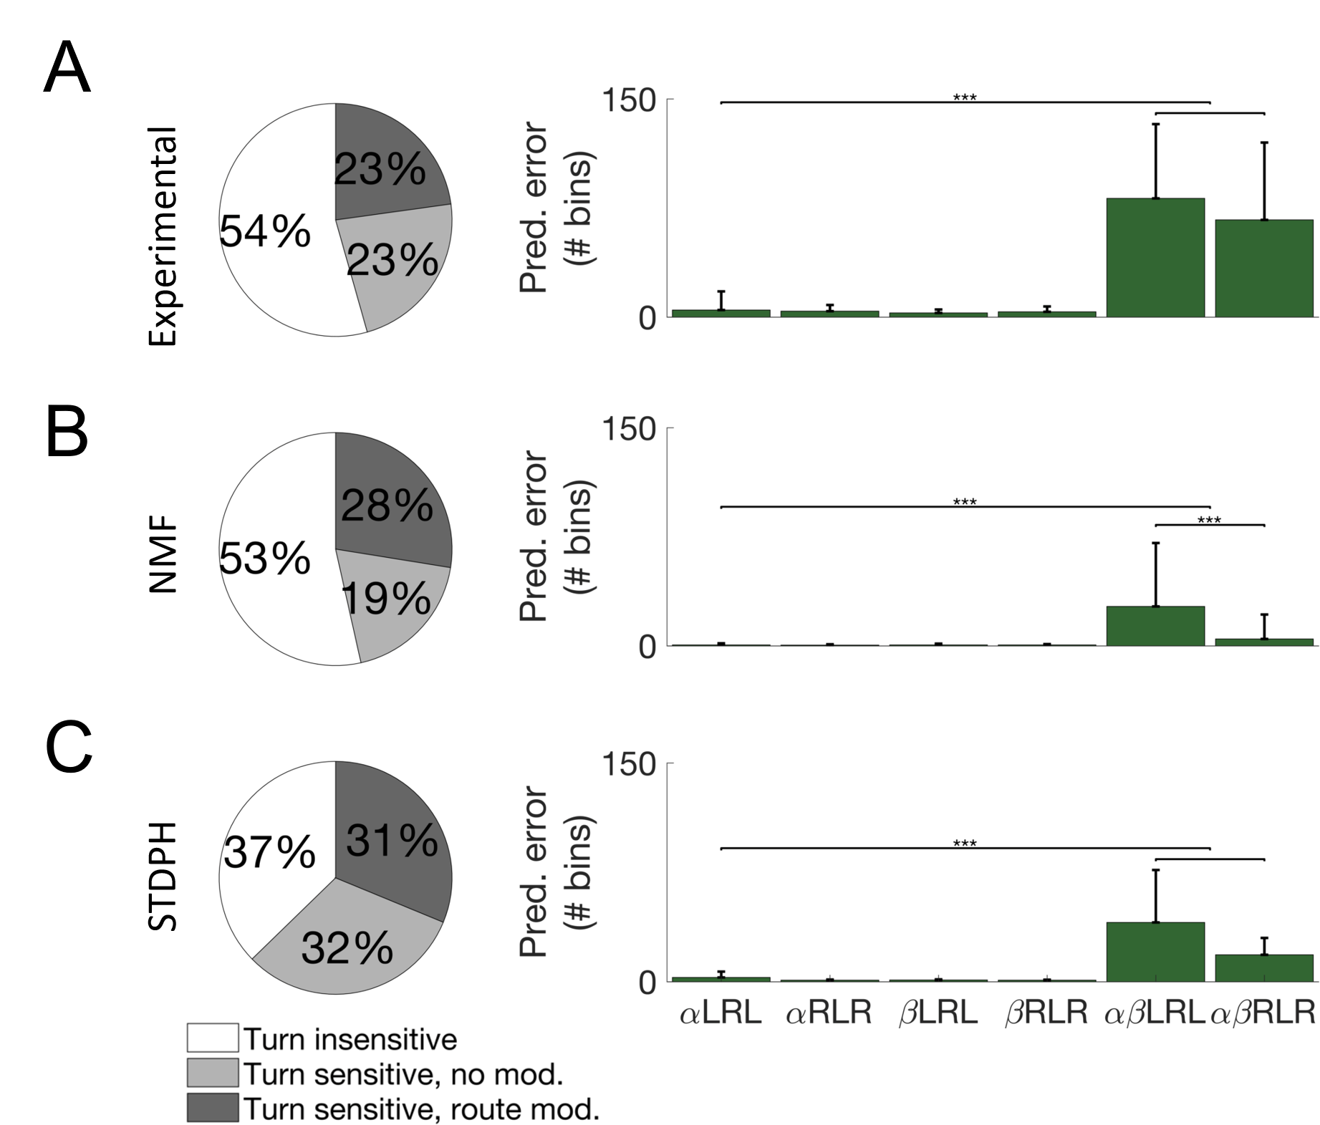
\includegraphics[width=\textwidth]{fig-rev1-rsc}
    \caption{Functional neuron type distributions found in the dataset and produced by each model (left columns) and average error corresponding to positional ensemble reconstruction matrices (right columns). Separate allocentric positions of the track are represented by the symbols $\alpha$ and $\beta$. Reconstructions between the track positions are represented by $\alpha$$\beta$. There were two possible routes associated with each track: an outbound run consisting of a left-right-left (LRL) turn sequence and an inbound run consisting of a right-left-right (RLR) turn sequence. A) Experimental data from \cite{AlexanderNitz2015}. B) Simulated using NMF. C) Simulated by evolving STDPH parameters to fit experimental data from \cite{Rounds2016}.}
	\label{fig:NMF|RSC}
\end{figure} 



These findings lend credence to our proposal that \ac{NMF} and \ac{STDPH} 
are functionally equivalent.
% REMOVE:
% Furthermore, the matrix \textbf{W} produced by \ac{NMF} when applied to the \ac{RSC} dataset was qualitatively similar to the synaptic weight matrices produced by 
% simulations in which \ac{STDPH} was evolved to match the same dataset.

% This evidence suggests that there is merit to comparing
% synaptic weights generated with both \ac{NMF} and \ac{STDPH} to
% synaptic connections in the brain.
% In cases where synaptic weights from biological neurons are unavailable,
% simulated weight matrices could be used to advance theories of brain areas 
% with complicated neuronal responses
% (such as \ac{MSTd} or \ac{RSC});
% for example, by predicting neuronal responses to novel stimuli
% and simulating experimental perturbations.


% \ac{NSC} may have emerged as a general encoding strategy is because it can be approximated by certain forms of synaptic plasticity, such as \ac{STDPH}, under certain conditions. STDP, or spike-timing dependent plasticity,\emilyNote{this sentence implies STDPH -> NSC, but relationship could be other way: NSC->STDPH, so be careful with this idea here...}
% %is a learning mechanism by which synaptic weights are potentiated or depressed based on the precise spike times of pre- and post-synapic neurons. \ac{STDP} 
% is a learning mechanism that has been found in many brain regions and is generally assumed to take place in some form in every brain region. \emilyNote{much citations, very need} However, there may be many kinds of implementations of STDP in the brain that could also impose other statistical constraints in addition to nonnegativity. In a modified \ac{STDPH} learning rule, STDP is complemented by a homeostatic synaptic scaling mechanism that may give rise to a biologically realistic implementation of \ac{NMF}. In this view, a specific synaptic weight
% (i.e., an element in \textbf{W})
% is modulated depending on the activity of a presynaptic neuron over time
% (i.e., a row in \textbf{V})
% and the activity of a postsynaptic neuron over time
% (i.e., a column in $\mathbf{H}^T$).
% Here, the dimension that used to encompass a number of observations or stimuli $S$
% is now interpreted as time $t$.
% In this context, a row of \textbf{V} corresponds to a specific neuron's firing
% rate over time.
% Then the synaptic weight update rule of \ac{STDPH}
% is mathematically equivalent to an iteration step in \ac{NMF}
% (see \citep{Carlson2013} for a mathematical proof).
% This bestows upon a pre-postsynaptic neuron pair the ability to implement
% \ac{NMF} literally through learning.\emilyNote{more citations; maybe kris would have some} This process is exemplified in Figure \ref{fig:NMF|STDPH}. However, there are multiple kinds of homeostasis that may exist in the brain as well, which may change the nature of the statistical constraints on the pre- and post-synaptic neuron pairs. 

% Another reason might be the fact that \ac{NMF} can be approximated
% by \ac{STDPH} \citep{Carlson2013} (Box 2).

% \mikeNote{words whole para}
% \Ac{STDP} is a synaptic learning that modulates synaptic weights based on the
% precise firing of pre and postsynaptic neurons.
% \Ac{STDP} is ubiquitous in the brain (even in the adult brain, right),
% but it comes in many different forms.
% In one particular form, where \ac{STDP} is complemented with
% homeostatic synaptic scaling (which we refer to as \ac{STDPH}),
% it might be equivalent to \ac{NMF}.



% In addition to nonnegativity constraints,  sparsity in the neural code may be enforced by lateral inhibitory connections in which excited neurons  inhibit their neighbors such that only a few neurons remain sufficiently active in response to a stimulus, resulting in enhanced  sensory perception. This kind of anti-Hebbian learning can be implemented using the Oja learning rule, which can then be used to control the sparsity of the neural code to ensure a robust and fault-tolerant, but also energy efficient, encoding. % Also Oja approximates PCA and that may or may not be relevant. 
% This conception of STDPH as a biological implementation of NMF implies that the weight matrices generated by an NMF decomposition should be equivalent to those learned by biological neurons in the brain, and by artificial neurons in SNNs under STDPH. Comparing the weight matrix \textbf{W} from \ac{NMF} once again
% to empirical data makes it clear that there is a strong correspondence, and in the case of \ac{V1}, synaptic weights recovered with \ac{NMF} closely resemble biological weight matrices in cat \ac{V1}. Moreover, similar results can be achieved with \ac{STDPH}. 
% %iffy on this
% The structures of synaptic weight matrices in higher cortical regions are unknown;
% \mikeNote{Sure, we can make this prediction. But it is not testable}
% however, we predict that comparisons of the matrix W generated by NMF and STDPH for the simulated RSC data would resemble the actual weight matrix associated with RSC neurons in the biological brain.



% \subsection{Retina}
% \label{sec:evidence|vision|retina}

% % Using \ac{NMF} to explain single-trial spike trains in the retina \citep{Onken2016}.

% % Overview:
% % - A variety of methods were applied to retinal ganglion cells  in order to analyze their firing patterns
% % - These methods included spatiotemporal PCA, ICA, and NMF, but also included Tucker-2 factorization with orthogonality or non-negativity constraints (yielding orthogonal Tucker-2 and space-by-time NMF).
% % - Space-by-time methods were more accurately able to decompose firing patterns into modules or basis vectors
% % - While orthogonal Tucker-2 was able to pick up on variance between patterns that allowed for better reconstruction (more efficient and more robust), space-by-time NMF picked up on stereotyped patterns and resulted in more consistent and generalizable modules
% % - (What does this actually mean...?)

% %  Means that for patterns of stimuli with spatial and temporal components, space-by-time techniques will be better at representing the underlying structure of the data. But if patterns are inseparable in space/time, then you don't need tensor factorization.
% % ...So what happens in the brain? Presumably both kinds of stimuli are possible. Does the brain have both spatiotemporal coding and tensor factorization style coding? What circumstances dictate when which is employed, if so?

% In seeking a scalable way to analyze population codes for large numbers of neurons in both the spatial and temporal dimensions, researchers applied spatiotemporal PCA, ICA, and NMF to both simulated spike trains and neurophysiological spike trains recorded from the retinas of salamanders. %Poor axolotls. :( 
% They also applied tensor factorization methods with either orthogonality or non-negativity constraints. Tensor factorization is a method that decomposes data into separated spatial and temporal domains such that you get separate basis functions (or "modules") for each. This is important because neurons may vary their responses in the spatial domain based on location (neurons closer to one another may share common inputs, for example), and in the temporal domain by varying their response patterns over time.  By decomposing firing rate patterns into spatial and temporal domains separately, a neuron's spatial and temporal contributions to the population code can be elucidated \citep{Onken2016}.

% The different techniques were applied to simplified simulated datasets in order to test how well each technique could extract the 'ground truth' of a known pattern, either separable or inseparable in space and time. First the researchers applied techniques to simulated datasets with a high signal to noise ratio (SNR) that were separable in space and time, which should be easily distinguishable. Blocks of time in which neurons fired at 300 Hz were randomly interspersed amongst background firing of only 2 Hz.  In this case, only spatiotemporal NMF and space by time NMF (Tucker-2 tensor factorization with non-negativity constraints) could recover the underlying ground truth in the pattern.  Given a low SNR (30 Hz with background firing of 2 Hz) pattern that was separable in space and time, only space-by-time NMF was able to faithfully recover the underlying structure. When a pattern was inseparable in space and time (SNR was again 300 Hz to 2 Hz), space by time NMF could no longer recover the underlying blocks, but spatiotemporal NMF could, suggesting that NMF is a better technique for decomposing firing rate data into its fundamental components than PCA or ICA.

% The researchers also looked at the differences between the Tucker-2 factorization methods with non-negativity or orthogonality constraints in their ability to recover stereotyped and repeated firing patterns in the data. They found that orthogonal Tucker-2 factorization led to more robust and efficient representations, but they were overall less compact, and they did not lead to stable modules that recovered stereotyped firing patterns - instead, this kind of factorization yielded modules that were less consistent and seemed to extract differences in activation pattern across stimuli (as opposed to commonalities). The authors note that all other methods with statistical constraints had the same inconsistency, suggesting that non-negativity is the most promising constraint for extracting stereotyped firing.

% Following testing on known ground truth, the researchers recorded spikes from in vitro retinal ganglion cells  while the cells were exposed to natural images (either still photographs or videos). They then applied the Tucker-2 factorization methods (with orthogonality or non-negativity constraints) to the recorded datasets. The results were similar to the simulated data case; space-by-time NMF could decompose the data into compact and sparse representations with three temporal modules and eight spatial modules, while orthogonal Tucker-2 yielded four temporal modulates and sixteen spatial modules. While orthogonal Tucker-2 was also more accurate than space-by-time NMF for correctly decoding the activity, the resulting modules were again inconsistent and relied more on differences between patterns of firing rather than extracting similarities in firing pattern. The modules resulting from space-by-time NMF, on the other hand, were more consistent and more representative of an underlying stereotyped pattern of firing in addition to being a sparser and more compact representation. 
% % Is it important to talk about the contribution of first spike latency and redundancy in spatial/temporal coding?

%  The researchers used the time-only and space-only information to decode the natural images presented to the RGCs and found that decoding was far less accurate when information from the spatial dimension was missing, but only slightly less accurate (though still statistically significantly so) when information from the temporal domain was missing. Further experiments using first spike latency (in which space-by-time NMF was applied to an altered dataset where all spikes except the first one for each neuron and trial were deleted) suggested that information is carried redundantly by spike timing and rate coding, because decoding error was on par with space-by-time NMF under these conditions. Further investigations in which RGCs were shown flashed gratings in different orientations revealed that spike timing is especially important for discriminating fine differences in images that fall within the boundaries of a receptive field.
 
%  The authors conclude that NMF is a biologically plausible tool for spike train analysis (the outputs of NMF can be directly interpreted as synaptic weights, and they are highly generalizable), and that the reason it has been used in a limited number of cases may be due to the fact that spatiotemporal NMF does not perform robustly under certain conditions; specifically, conditions where there is significant overlap in firing patterns and when there is a low SNR. By using space-by-time NMF, these problems can be overcome, and also allows for the analysis of the spatiotemporal structure of neuronal firing patterns. We suggest that the good performance of space-by-time NMF in terms of its ability to extract a sparse and highly compact representation of the underlying structure of a neural code is further evidence that the brain may be employing similar methods for handling the high dimensionality of incoming stimuli. However, since not all patterns are separable in space and time, it is an open question how the brain might handle incoming information under such conditions.

% "The advantage of the non-negative decomposition was its ability to robustly find compact and directly interpretable firing patterns that occur across many different kinds of stimuli. These patterns can be used as basis functions to linearly build a set of code-words of firing patterns, complementing existing approaches [98, 99]. The shape of these firing patterns can thus be examined to provide important information about the structure of the neural code, for example to make hypotheses about the spatial and temporal resolution at which a neural code should be read out. As an example of the information that these modules may give, the structure of spatial modules extracted from RGCs suggests that informative patterns of simultaneous firing come from localized groups of neurons whose receptive fields are close together and that have similar stimulus tuning. "




% \subsection{Early visual cortex}
% \label{sec:evidence|vision|V1}
% % MB TODO

% A popular theory about early visual cortex function is that of sparse coding.

% Sparsity has been proposed as a general principle for the visual cortex. Barlow has argued for sparsity
% on the grounds that only a small proportion of neurons in V1 (and elsewhere??) fire in response to a
% given image and hence the response is ”sparse”. This is desirable for neurons because it means that only
% a few of them need to be active and expend energy (the brain consumes more energy than the rest of the
% body).

% The principle behind sparse coding is that the vision system has an over-complete set of basis functions.
% It tries to represent each image in terms of a small set of these functions. This over-completeness means
% that the the basis functions can be tuned to interesting features of the image. As mentioned above, the
% sparsity principle can also be used to learn receptive fields from natural images (refs!!).

% This sparsity criteria was developed by Olshausen and Field as a way to learn receptive fields of
% neurons \citep{OlshausenField1996}. It gives a reconstruction criteria that can be extended to multiple images and used to learn receptive fields.

% This results in receptive field models which are similar to those measured \citep{OlshausenField1996}. Note that similar
% receptive fields can be obtained by assuming a similar model for the image, see equation (7), but imposing
% different assumptions on the form of the si
% . In particular, independent component analysis (ICA) gives
% similar receptive field models \citep{vanHateren1998}.
% \cite{Hyvarinen2010} explained this by showing that both types of models –
% L1 sparsity and \ac{ICA} – both encourage that the $s_i$ are strongly peaked at 0, 
% but can occasionally have
% large non-zero values (this contrasts with the Gaussian model – e.g. pseudo-inverse – where the 
% $s_i$ are strongly discouraged from taking large values).



% % Topographic NMF: \url{http://www.mitpressjournals.org/doi/pdf/10.1162/neco.2009.03-08-722}
% % It seems like they're adding space to the NMF computation, which might make this kind of similar to the space-by-time NMF algorithm discussed in the retina paper? Am I thinking about that correctly? -Emily






% \subsection{Audition}
% \url{https://www.ncbi.nlm.nih.gov/pmc/articles/PMC4747712/}
% Wondering if NMF could explain the feature composition

% \subsection{Speech}
% S. Zayd Enam, Michael R. DeWeese: Spectro-Temporal Models of Inferior Colliculus Neuron Receptive Fields 
% Sparse codes for speech spectrograms qualitatively match properties of receptive fields of Inferior Colliculus (ICC) neurons. We find sparse codes of speech-spectrograms are well described by one of four models and we find that these models also fit ICC spectro-temporal receptive fields (STRF) well. Further, our models are able to express time-frequency inseparable receptive fields (e.g. frequency sweeps) that previous models were unable to satisfactorily describe. Our models allow the accurate characterization of high-dimensional STRFs with more natural parameterizations of the neuron's behavior. \emilyNote{Not sure we'd want to cite this paper? "To determine STRF model classes we first fit model classes to the sparse codes of speech-spectrograms using non-linear least squares methods"}


% \subsection{Olfaction}

% % Structure this as...
% % 1) There are lots of possible odor combinations and sparse ensemble of neurons to encode them
% % 2) The sparsity of the olfactory code is poor in information and metabolically costly, so functional significance is unclear
% % 3)  Granule cells may complement the code of the mitral cells because they are sparse/incomplete representations
% % 4) This might result in 'explaining away' approach by this system as described in the SNN paper, which was able to detect combinations of odorants very accurately
% % 5) Brief description of causal inference in spiking via explaining away and how it relates to NMF?


% Check this Drugowitsch paper:
% Causal Inference and Explaining Away in a Spiking Network
% Rubén Moreno-Bote \& Jan Drugowitsch, Scientific Reports
% \url{https://www.nature.com/articles/srep17531}

% Also Koulakov and Rinberg:
% Sparse incomplete representations: A novel role for olfactory granule cells
% \url{https://pdfs.semanticscholar.org/ed52/1b318aa68fe8ec71fb9a84d5e577130c6893.pdf}

% It's \emph{almost} doing \ac{NMF},
% and suggests that such a computation might underlie odor classification.

% Antennae -> antennal lobe -> mushroom body (Kenyan cell)
% only 34 output neurons for odor classification
% any given odor activates a unique and sparse ensemble of kenyan cells

% From Graziano \& Aflalo: In this review, the authors suggest that at least some sectors of the cortex do not have a simple global ordering and are better understood as a result of a reduction of a highdimensional space onto the cortical sheet. The cortical motor system may be an example of this phenomenon. The authors discuss a model of the lateral motor cortex in which a reduction of many parameters onto a simulated cortical sheet results in a complex topographic pattern that matches the actual monkey motor cortex in surprising detail. \citep{GrazianoAflalo2007} Source:

% \url{https://www.princeton.edu/~graziano/neuroscientist_07.pdf}
% \url{http://ieeexplore.ieee.org/document/7229368}


% % \subsection{Somatosensory cortex}
% % % MB probably cut...

% % Chapin \& Nicolelis (1999). Journal of Neuroscience Methods. Principal component analysis of neuronal ensemble activity reveals multidimensional somatosensory representations.
% % Recorded neurons from rat somatosensory cortex and applied PCA to the data. Found multidimensional somatosensory receptive fields.
% % From abstract: "The fact that this transformation is mathematically equivalent to the general Hebb algorithm in linear neural networks provided a major rationale for performing it here on data from real neuronal ensembles."


\section*{\revise{Limitations of NSC and alternatives}}
\label{sec:limitations}

\mikeNote{Reviewer 2 wants us to discuss all these limitations and compare NSC to other theories. We could do this in the Conclusions, but I thought a Limitations section right before the end would make more sense, so that we can end the paper on a high note with positive conclusions.

Here's a potential outline for this section. Just needs more sciency words.}

\revise{The role of sparse coding has been questioned in the brain 
\cite{SpanneJorntell2015}.
One issue that basically any code between local and dense can be labeled sparse
\cite{SpanneJorntell2015}. That's not a big deal because we're fine with that definition. We find it interesting that there is a sweet spot for the sparsity of the code, depending on population size and the complexity of the information that is being encoded. We previously showed this for \ac{MSTd} \cite{Beyeler2016}.
We have no doubt that the sparsity of the code might differ in different areas. For example, \ac{V1} seems to operate in a regime with an overcomplete basis set \cite{olshausen1997}. On the other hand, \ac{MSTd} seems to operate with a relatively small dictionary. We think this gives \ac{MSTd} an increased representational capacity which could lead to compact and multifaceted encodings of various perceptual variables
(see Discussion in \cite{Beyeler2016}).}

\revise{Then some people have questioned whether some regions are really sparse.
For one, there are the two examples raised in the Spanne article: basal ganglia and different layers of visual cortex. Turns out basal ganglia might not be too sparse. Turns out only Layer 2/3 in V1 might be sparse.}

\revise{The problem is that there is a problem with simulation studies:
If you study simple phenomena, you might get simple dynamics (this addresses a comment
by Reviewer 1). There's not much you can do, except focus on all attributes of the
population code, not just sparsity.
From Gao \cite{Gao2017}: Dimensionality reduction methods reveal a striking simplicity underlying such multi-neuronal data: they can be reduced to a low-dimensional space, and the resulting neural trajectories in this space yield a remarkably insightful dynamical portrait of circuit computation. This simplicity raises profound and timely conceptual questions. What are its origins and its implications for the complexity of neural dynamics? How would the situation change if we recorded more neurons? When, if at all, can we trust dynamical portraits obtained from measuring an infinitesimal fraction of task relevant neurons?}


\revise{Finally, there are other competing theories of brain function, 
such as compressed sensing \cite{GanguliSompolinsky2012}.
Compressed sensing works like this and that.
There's also predictive coding and free energy and blah blah blah,
but we don't want to talk about everyone and their grandmother.}

\revise{This leads to our final point: that we don't think the brain the does NSC
and only NSC.
This is just something we want to stress to please the reviewers.
We simply highlight NSC as a potential canonical computation - we found it pop up all
over the brain and are intrigued. However, we need more research to see this through.}



\section*{\revise{Conclusion}}
\label{sec:conclusion}

\revise{In conclusion,
there is increasing evidence that \ac{NSC} can account for a wide variety of
neuronal response properties especially in sensory and associative cortices.
Although \ac{NSC} might not apply to the motor system,
its success warrants further investigation.}

\section*{Acknowledgments}

Supported by the National Science Foundation (Award IIS-1302125) and the Washington Research Foundation Funds for Innovation in Neuroengineering and Data-Intensive Discovery (M.B.).

\nolinenumbers

\bibliography{references}

\linenumbers

% Ok, so apparently the glossary isn't just a list of all acronyms
% Pick a few central terms that are worth explaining
% Limit to 450 words

\section*{Glossary}
\label{sec:Glossary}

\begin{itemize}
% list alphabetically
% term in bold, then explain more than just long version of abbreviation
\item \textbf{Allocentric reference frame} \mikeNote{Really needed? not important enough} A spatial frame of reference that is defined with respect to a broader environment (e.g., one's location on a map). Hippocampal place cells are a textbook example of neurons that are anchored to an allocentric reference frame.

\item \textbf{Basis functions} \mikeNote{Really needed? not important enough} A lower-dimensional set of linearly independent elements that can represent a high-dimensional input space given a weighted sum of these elements, where the weight of each element is defined by a separate hidden component.

% \item \textbf{Binary tournament selection} A selection strategy for producing new parents for the next generation in an evolutionary strategy. In tournament selection, $x$ individuals are chosen randomly, and then the individual in the subset with the highest fitness is chosen as a parent. This is repeated until the number of desired parents have been chosen. In binary tournament selection, $x = 2$ individuals are chosen at random from the population.

% \item \textbf{Crossover} In an evolutionary strategy, parents chosen to produce the next generation may undergo crossover. Each parent has a value associated with each parameter being evolved. To produce a child, the values associated with a parameter may be swapped at random (using a predetermined threshold) between the parents so that the child has a mixture of both parents' parameter values.

\item \textbf{Dimensionality reduction} The process of reducing the dimensionality of a space to the lowest possible space that encapsulates the variance of the original data via feature extraction. In the case of neuronal firing rate patterns, this means representing all possible firing rate patterns in the brain region using the smallest possible subset of the neurons.

\item \textbf{Efficient coding} TODO

\item \textbf{Egocentric reference frame} \mikeNote{Really needed? not really important} A spatial frame of reference that is defined with respect to one's own perspective (e.g., taking a left turn is an action performed with respect to the egocentric reference frame).

\item \textbf{Factor analysis} \mikeNote{Really needed? not really important} A statistical method used to describe variability among observed, correlated variables in terms of a potentially lower number of unobserved, uncorrelated variables called factors (or latent variables).

% \item \textbf{Fitness} In evolutionary strategies, a single value computed with a user-defined function that represents how well an individual in a population meets the desired function that is being evolved.

\item \textbf{\Acf{ICA}} TODO

% \item \textbf{Mutation} In an evolutionary strategy, parents chosen to produce the next generation may undergo mutation. Each parent has a value associated with each parameter being evolved. Each parameter may be randomly altered (according to a predetermined threshold) by selecting a new value from some distribution of values that lie within the established range to produce a new child individual for the next generation.

\item \textbf{\Acf{PCA}} TODO

\item \textbf{Receptive field} \mikeNote{Really needed? they're biologists} The structure and boundaries of an individual neuron's pattern of response to various kinds of incoming stimuli.

\item \textbf{Representational capacity} The ability to represent information depends on the number of recognizably different patterns of neuronal activity that can be generated in a useful time interval. This number---the representational capacity---is a fundamental measure of neural performance \cite{Laughlin2001}.

\item \textbf{Route-centric reference frame} \mikeNote{Really needed? not really important} A spatial frame of reference that is defined with respect to a planned path through a broader environment. For example, neurons in some parts of the brain fire for a particular location in a route, even if the route is repositioned or reoriented in the broader environment \cite{nitz2009parietal}.

\item \textbf{Sparse coding} TODO.

\item \textbf{Spike-timing dependent plasticity} \mikeNote{Really needed? they're biologists} A Hebbian-inspired learning rule in which weight updates are computed based on the precise spike times of pre- and post-synaptic neurons that induce either long term potentiation or long term depression in the synapse, depending on whether the total pre-synaptic spike count preceded the total post-synaptic spike count, integrated over a critical temporal window.

\end{itemize}
\section*{\revise{Supplementary Material}}
\label{sec:SupplementaryMaterial}
\subsubsection*{\revise{Details of experiments in retrosplenial cortex.}}

\revise{Alexander and Nitz \cite{AlexanderNitz2015} investigated the spatial reference frame(s) to which retrosplenial cortical activity is anchored. In their experiments, six Long-Evans rats traversed a W-shaped track that occupied two distinct positions in the recording room, referred to as track positions $\alpha$ and $\beta$, which varied by recording session. The track was composed of two sets of action sequences depending on the direction of traversal (outbound or inbound trials). Outbound and inbound runs were made up of opposite turn sequences (left-right-left (LRL) and right-left-right (RLR), respectively. The manipulation of turn sequence, route, and track position allowed the assessment of neural sensitivity to the \textit{allocentric}, \textit{egocentric} and \textit{route-based} reference frames by comparing the observed firing patterns of electrophysiologically recorded neurons by the rat's position with respect to the route, the room, and the action being performed. In total, 243 neurons were recorded over 71 recording sessions, with measures taken to ensure maximum independence between the neurons that were recorded in each session. Each session had approximately 20 trials per condition (track position by direction of traversal). Additionally, Alexander and Nitz \cite{AlexanderNitz2015} recorded relevant behavioral data concurrently with neuronal firing patterns for each trial, including head direction (HD), position in X-Y coordinates (Pos), linear velocity (LV), and angular velocity (AV).}

\revise{Using the experimental data collected in these experiments, Rounds et al. \cite{Rounds2016,Rounds2018} used an evolutionary strategy to evolve a population of spiking neural networks (SNNs) that could replicate the functional, behavioral, and population responses observed in the electrophysiologically recorded data in response to the recorded behavioral metrics HD, Pos, LV, and AV. Each network contained 600 neurons (480 excitatory and 120 inhibitory Izhikevich neurons \cite{izhikevich2003simple}). Each trial consisted of 200 bins, each associated with a specific combination of these four inputs. The recorded values were encoded using cosine and Gaussian tuning curves that were subjected to a Poisson process to produce spiking inputs. The population was allowed to evolve over 50 generations, with convergence occurring by approximately the 20th generation. Synthetic neural activity was averaged across trials for each track position/traversal combination and then correlated with the 243 electrophysiologically recorded neuronal firing patterns. For each of the electrophysiologically recorded neurons, the synthetic neuron with the highest-correlated firing pattern was assigned as a match for that neuron. No duplicate matches were allowed - a neuron could be matched only once. Each SNN in the population was evaluated according to a fitness function that measured the sum of the highest correlations between neurons, with a penalty for overly high average maximum firing rates for the synthetic neurons to ensure a stable firing regime. The networks consistently converged to a fitness value of 105.93 $\pm$ 0.91 (arbitrary units), or an average correlation of Pearson's \textit{R} = 0.43 per neuron (high correlations by experimental standards). For further details on experimental methods, see \cite{AlexanderNitz2015,Rounds2016,Rounds2018}.}


\end{document}